\documentclass[10pt,compress,t,notes=noshow, xcolor=table]{beamer}

\usepackage[]{graphicx}
% graphicx is loaded via lmu-lecture.sty as well
\usepackage[]{color}
% maxwidth is the original width if it is less than linewidth
% otherwise use linewidth (to make sure the graphics do not exceed the margin)
\makeatletter
\def\maxwidth{ %
  \ifdim\Gin@nat@width>\linewidth
    \linewidth
  \else
    \Gin@nat@width
  \fi
}
\makeatother

% ---------------------------------%
% latex-math dependencies, do not remove:
% - mathtools
% - bm
% - siunitx
% - dsfont
% - xspace
% ---------------------------------%

%--------------------------------------------------------%
%       Language, encoding, typography
%--------------------------------------------------------%

\usepackage[english]{babel}
\usepackage[utf8]{inputenc} % Enables inputting UTF-8 symbols
% Standard AMS suite (loaded via lmu-lecture.sty)
\usepackage{amsmath,amsfonts,amssymb}

% Font for double-stroke / blackboard letters for sets of numbers (N, R, ...)
% Distribution name is "doublestroke"
% According to https://mirror.physik.tu-berlin.de/pub/CTAN/fonts/doublestroke/dsdoc.pdf
% the "bbm" package does a similar thing and may be superfluous.
% Required for latex-math
\usepackage{dsfont}

% bbm – "Blackboard-style" cm fonts (https://www.ctan.org/pkg/bbm)
% Used to be in common.tex, loaded directly after this file
% Maybe superfluous given dsfont is loaded
% TODO: Check if really unused?
% \usepackage{bbm}

% bm – Access bold symbols in maths mode - https://ctan.org/pkg/bm
% Required for latex-math, preferred over \boldsymbol
% https://tex.stackexchange.com/questions/3238/bm-package-versus-boldsymbol
\usepackage{bm}

% pifont – Access to PostScript standard Symbol and Dingbats fonts
% Used for \newcommand{\xmark}{\ding{55}, which is never used
% aside from lecture_advml/attic/xx-automl/slides.Rnw
% \usepackage{pifont}

% Quotes (inline and display), provdes \enquote
% https://ctan.org/pkg/csquotes
\usepackage{csquotes}

% Adds arg to enumerate env, technically superseded by enumitem according
% to https://ctan.org/pkg/enumerate
% Replace with https://ctan.org/pkg/enumitem ?
% Even better: enumitem is not really compatible with beamer and breaks all sorts of things
% particularly the enumerate environment. The enumerate package also just isn't required
% from what I can tell so... don't re-add it I guess?
% \usepackage{enumerate}

% Line spacing - provides \singlespacing \doublespacing \onehalfspacing
% https://ctan.org/pkg/setspace
% \usepackage{setspace}

% mathtools – Mathematical tools to use with amsmath
% https://ctan.org/pkg/mathtools?lang=en
% latex-math dependency according to latex-math repo
\usepackage{mathtools}

% Maybe not great to use this https://tex.stackexchange.com/a/197/19093
% Use align instead -- TODO: Global search & replace to check, eqnarray is used a lot
% $ rg -f -u "\begin{eqnarray" -l | grep -v attic | awk -F '/' '{print $1}' | sort | uniq -c
%   13 lecture_advml
%   14 lecture_i2ml
%    2 lecture_iml
%   27 lecture_optimization
%   45 lecture_sl
\usepackage{eqnarray}

% For shaded regions / boxes
% Used sometimes in optim
% https://www.ctan.org/pkg/framed
\usepackage{framed}

%--------------------------------------------------------%
%       Cite button (version 2024-05)
%--------------------------------------------------------%
% Note this requires biber to be in $PATH when running,
% telltale error in log would be e.g. Package biblatex Info: ... file 'authoryear.dbx' not found
% aside from obvious "biber: command not found" or similar.
% Tried moving this to lmu-lecture.sty but had issues I didn't quite understood,
% so it's here for now.

\usepackage{textcase} % for \NoCaseChange
\usepackage{hyperref}

% Only try adding a references file if it exists, otherwise
% this would compile error when references.bib is not found
\IfFileExists{references.bib} {
  \usepackage{usebib}
  \usepackage[backend=biber, style=authoryear]{biblatex}

  \addbibresource{./references.bib}
  \bibinput{references}
}

\newcommand{\citelink}[1]{%
\NoCaseChange{\resizebox{!}{9pt}{\protect\beamergotobutton{\href{\usebibentry{\NoCaseChange{#1}}{url}}{\begin{NoHyper}\cite{#1}\end{NoHyper}}}}}%
}

%--------------------------------------------------------%
%       Displaying code and algorithms
%--------------------------------------------------------%

% Reimplements verbatim environments: https://ctan.org/pkg/verbatim
% verbatim used sed at least once in
% supervised-classification/slides-classification-tasks.tex
% Removed since code should not be put on slides anyway
% \usepackage{verbatim}

% Both used together for algorithm typesetting, see also overleaf: https://www.overleaf.com/learn/latex/Algorithms
% algorithmic env is also used, but part of the bundle:
%   "algpseudocode is part of the algorithmicx bundle, it gives you an improved version of algorithmic besides providing some other features"
% According to https://tex.stackexchange.com/questions/229355/algorithm-algorithmic-algorithmicx-algorithm2e-algpseudocode-confused
\usepackage{algorithm}
\usepackage{algpseudocode}

%--------------------------------------------------------%
%       Tables
%--------------------------------------------------------%

% multi-row table cells: https://www.namsu.de/Extra/pakete/Multirow.html
% Provides \multirow
% Used e.g. in evaluation/slides-evaluation-measures-classification.tex
\usepackage{multirow}

% colortbl: https://ctan.org/pkg/colortbl
% "The package allows rows and columns to be coloured, and even individual cells." well.
% Provides \columncolor and \rowcolor
% \rowcolor is used multiple times, e.g. in knn/slides-knn.tex
\usepackage{colortbl}

% long/multi-page tables: https://texdoc.org/serve/longtable.pdf/0
% Not used in slides
% \usepackage{longtable}

% pretty table env: https://ctan.org/pkg/booktabs
% Is used
% Defines \toprule
\usepackage{booktabs}

%--------------------------------------------------------%
%       Figures: Creating, placing, verbing
%--------------------------------------------------------%

% wrapfig - Wrapping text around figures https://de.overleaf.com/learn/latex/Wrapping_text_around_figures
% Provides wrapfigure environment -used in lecture_optimization
\usepackage{wrapfig}

% Sub figures in figures and tables
% https://ctan.org/pkg/subfig -- supersedes subfigure package
% Provides \subfigure
% \subfigure not used in slides but slides-tuning-practical.pdf errors without this pkg, error due to \captionsetup undefined
\usepackage{subfig}

% Actually it's pronounced PGF https://en.wikibooks.org/wiki/LaTeX/PGF/TikZ
\usepackage{tikz}

% No idea what/why these settings are what they are but I assume they're there on purpose
\usetikzlibrary{shapes,arrows,automata,positioning,calc,chains,trees, shadows}
\tikzset{
  %Define standard arrow tip
  >=stealth',
  %Define style for boxes
  punkt/.style={
    rectangle,
    rounded corners,
    draw=black, very thick,
    text width=6.5em,
    minimum height=2em,
    text centered},
  % Define arrow style
  pil/.style={
    ->,
    thick,
    shorten <=2pt,
    shorten >=2pt,}
}

%--------------------------------------------------------%
%       Beamer setup and custom macros & environments
%--------------------------------------------------------%

% Main sty file for beamer setup (layout, style, lecture page numbering, etc.)
% For long-term maintenance, this may me refactored into a more modular set of .sty files
\usepackage{../../style/lmu-lecture}
% Custom itemize wrappers, itemizeS, itemizeL, etc
\usepackage{../../style/customitemize}
% Custom framei environment, uses custom itemize!
\usepackage{../../style/framei}
% Custom frame2 environment, allows specifying font size for all content
\usepackage{../../style/frame2}
% Column layout macros
\usepackage{../../style/splitV} 

% Used regularly
\let\code=\texttt

% Not sure what/why this does
\setkeys{Gin}{width=0.9\textwidth}

% -- knitr leftovers --
% Used often in conjunction with \definecolor{shadecolor}{rgb}{0.969, 0.969, 0.969}
% Removing definitions requires chaning _many many_ slides, which then need checking to see if output still ok
\definecolor{fgcolor}{rgb}{0.345, 0.345, 0.345}
\definecolor{shadecolor}{rgb}{0.969, 0.969, 0.969}
\newenvironment{knitrout}{}{} % an empty environment to be redefined in TeX

%-------------------------------------------------------------------------------------------------------%
%  Unused stuff that needs to go but is kept here currently juuuust in case it was important after all  %
%-------------------------------------------------------------------------------------------------------%

% \newcommand{\hlnum}[1]{\textcolor[rgb]{0.686,0.059,0.569}{#1}}%
% \newcommand{\hlstr}[1]{\textcolor[rgb]{0.192,0.494,0.8}{#1}}%
% \newcommand{\hlcom}[1]{\textcolor[rgb]{0.678,0.584,0.686}{\textit{#1}}}%
% \newcommand{\hlopt}[1]{\textcolor[rgb]{0,0,0}{#1}}%
% \newcommand{\hlstd}[1]{\textcolor[rgb]{0.345,0.345,0.345}{#1}}%
% \newcommand{\hlkwa}[1]{\textcolor[rgb]{0.161,0.373,0.58}{\textbf{#1}}}%
% \newcommand{\hlkwb}[1]{\textcolor[rgb]{0.69,0.353,0.396}{#1}}%
% \newcommand{\hlkwc}[1]{\textcolor[rgb]{0.333,0.667,0.333}{#1}}%
% \newcommand{\hlkwd}[1]{\textcolor[rgb]{0.737,0.353,0.396}{\textbf{#1}}}%
% \let\hlipl\hlkwb

% \makeatletter
% \newenvironment{kframe}{%
%  \def\at@end@of@kframe{}%
%  \ifinner\ifhmode%
%   \def\at@end@of@kframe{\end{minipage}}%
%   \begin{minipage}{\columnwidth}%
%  \fi\fi%
%  \def\FrameCommand##1{\hskip\@totalleftmargin \hskip-\fboxsep
%  \colorbox{shadecolor}{##1}\hskip-\fboxsep
%      % There is no \\@totalrightmargin, so:
%      \hskip-\linewidth \hskip-\@totalleftmargin \hskip\columnwidth}%
%  \MakeFramed {\advance\hsize-\width
%    \@totalleftmargin\z@ \linewidth\hsize
%    \@setminipage}}%
%  {\par\unskip\endMakeFramed%
%  \at@end@of@kframe}
% \makeatother

% \definecolor{shadecolor}{rgb}{.97, .97, .97}
% \definecolor{messagecolor}{rgb}{0, 0, 0}
% \definecolor{warningcolor}{rgb}{1, 0, 1}
% \definecolor{errorcolor}{rgb}{1, 0, 0}
% \newenvironment{knitrout}{}{} % an empty environment to be redefined in TeX

% \usepackage{alltt}
% \newcommand{\SweaveOpts}[1]{}  % do not interfere with LaTeX
% \newcommand{\SweaveInput}[1]{} % because they are not real TeX commands
% \newcommand{\Sexpr}[1]{}       % will only be parsed by R
% \newcommand{\xmark}{\ding{55}}%

% textpos – Place boxes at arbitrary positions on the LATEX page
% https://ctan.org/pkg/textpos
% Provides \begin{textblock}
% TODO: Check if really unused?
% \usepackage[absolute,overlay]{textpos}

% -----------------------%
% Likely knitr leftovers %
% -----------------------%

% psfrag – Replace strings in encapsulated PostScript figures
% https://www.overleaf.com/latex/examples/psfrag-example/tggxhgzwrzhn
% https://ftp.mpi-inf.mpg.de/pub/tex/mirror/ftp.dante.de/pub/tex/macros/latex/contrib/psfrag/pfgguide.pdf
% Can't tell if this is needed
% TODO: Check if really unused?
% \usepackage{psfrag}

% arydshln – Draw dash-lines in array/tabular
% https://www.ctan.org/pkg/arydshln
% !! "arydshln has to be loaded after array, longtable, colortab and/or colortbl"
% Provides \hdashline and \cdashline
% Not used in slides
% \usepackage{arydshln}

% tabularx – Tabulars with adjustable-width columns
% https://ctan.org/pkg/tabularx
% Provides \begin{tabularx}
% Not used in slides
% \usepackage{tabularx}

% placeins – Control float placement
% https://ctan.org/pkg/placeins
% Defines a \FloatBarrier command
% TODO: Check if really unused?
% \usepackage{placeins}

% Can't find a reason why common.tex is not just part of this file?
% This file is included in slides and exercises

% Rarely used fontstyle for R packages, used only in 
% - forests/slides-forests-benchmark.tex
% - exercises/single-exercises/methods_l_1.Rnw
% - slides/cart/attic/slides_extra_trees.Rnw
\newcommand{\pkg}[1]{{\fontseries{b}\selectfont #1}}

% Spacing helpers, used often (mostly in exercises for \dlz)
\newcommand{\lz}{\vspace{0.5cm}} % vertical space (used often in slides)
\newcommand{\dlz}{\vspace{1cm}}  % double vertical space (used often in exercises, never in slides)
\newcommand{\oneliner}[1] % Oneliner for important statements, used e.g. in iml, algods
{\begin{block}{}\begin{center}\begin{Large}#1\end{Large}\end{center}\end{block}}

% Don't know if this is used or needed, remove?
% textcolor that works in mathmode
% https://tex.stackexchange.com/a/261480
% Used e.g. in forests/slides-forests-bagging.tex
% [...] \textcolor{blue}{\tfrac{1}{M}\sum^M_{m} [...]
% \makeatletter
% \renewcommand*{\@textcolor}[3]{%
%   \protect\leavevmode
%   \begingroup
%     \color#1{#2}#3%
%   \endgroup
% }
% \makeatother


% dependencies: amsmath, amssymb, dsfont
% math spaces
\ifdefined\N
\renewcommand{\N}{\mathds{N}} % N, naturals
\else \newcommand{\N}{\mathds{N}} \fi
\newcommand{\Z}{\mathds{Z}} % Z, integers
\newcommand{\Q}{\mathds{Q}} % Q, rationals
\newcommand{\R}{\mathds{R}} % R, reals
\ifdefined\C
\renewcommand{\C}{\mathds{C}} % C, complex
\else \newcommand{\C}{\mathds{C}} \fi
\newcommand{\continuous}{\mathcal{C}} % C, space of continuous functions
\newcommand{\M}{\mathcal{M}} % machine numbers
\newcommand{\epsm}{\epsilon_m} % maximum error

% counting / finite sets
\newcommand{\setzo}{\{0, 1\}} % set 0, 1
\newcommand{\setmp}{\{-1, +1\}} % set -1, 1
\newcommand{\unitint}{[0, 1]} % unit interval

% basic math stuff
\newcommand{\xt}{\tilde x} % x tilde
\DeclareMathOperator*{\argmax}{arg\,max} % argmax
\DeclareMathOperator*{\argmin}{arg\,min} % argmin
\newcommand{\argminlim}{\mathop{\mathrm{arg\,min}}\limits} % argmax with limits
\newcommand{\argmaxlim}{\mathop{\mathrm{arg\,max}}\limits} % argmin with limits
\newcommand{\sign}{\operatorname{sign}} % sign, signum
\newcommand{\I}{\mathbb{I}} % I, indicator
\newcommand{\order}{\mathcal{O}} % O, order
\newcommand{\bigO}{\mathcal{O}} % Big-O Landau
\newcommand{\littleo}{{o}} % Little-o Landau
\newcommand{\pd}[2]{\frac{\partial{#1}}{\partial #2}} % partial derivative
\newcommand{\floorlr}[1]{\left\lfloor #1 \right\rfloor} % floor
\newcommand{\ceillr}[1]{\left\lceil #1 \right\rceil} % ceiling
\newcommand{\indep}{\perp \!\!\! \perp} % independence symbol

% sums and products
\newcommand{\sumin}{\sum\limits_{i=1}^n} % summation from i=1 to n
\newcommand{\sumim}{\sum\limits_{i=1}^m} % summation from i=1 to m
\newcommand{\sumjn}{\sum\limits_{j=1}^n} % summation from j=1 to p
\newcommand{\sumjp}{\sum\limits_{j=1}^p} % summation from j=1 to p
\newcommand{\sumik}{\sum\limits_{i=1}^k} % summation from i=1 to k
\newcommand{\sumkg}{\sum\limits_{k=1}^g} % summation from k=1 to g
\newcommand{\sumjg}{\sum\limits_{j=1}^g} % summation from j=1 to g
\newcommand{\summM}{\sum\limits_{m=1}^M} % summation from m=1 to M
\newcommand{\meanin}{\frac{1}{n} \sum\limits_{i=1}^n} % mean from i=1 to n
\newcommand{\meanim}{\frac{1}{m} \sum\limits_{i=1}^m} % mean from i=1 to n
\newcommand{\meankg}{\frac{1}{g} \sum\limits_{k=1}^g} % mean from k=1 to g
\newcommand{\meanmM}{\frac{1}{M} \sum\limits_{m=1}^M} % mean from m=1 to M
\newcommand{\prodin}{\prod\limits_{i=1}^n} % product from i=1 to n
\newcommand{\prodkg}{\prod\limits_{k=1}^g} % product from k=1 to g
\newcommand{\prodjp}{\prod\limits_{j=1}^p} % product from j=1 to p

% linear algebra
\newcommand{\one}{\bm{1}} % 1, unitvector
\newcommand{\zero}{\mathbf{0}} % 0-vector
\newcommand{\id}{\bm{I}} % I, identity
\newcommand{\diag}{\operatorname{diag}} % diag, diagonal
\newcommand{\trace}{\operatorname{tr}} % tr, trace
\newcommand{\spn}{\operatorname{span}} % span
\newcommand{\scp}[2]{\left\langle #1, #2 \right\rangle} % <.,.>, scalarproduct
\newcommand{\mat}[1]{\begin{pmatrix} #1 \end{pmatrix}} % short pmatrix command
\newcommand{\Amat}{\mathbf{A}} % matrix A
\newcommand{\Deltab}{\mathbf{\Delta}} % error term for vectors

% basic probability + stats
\renewcommand{\P}{\mathds{P}} % P, probability
\newcommand{\E}{\mathds{E}} % E, expectation
\newcommand{\var}{\mathsf{Var}} % Var, variance
\newcommand{\cov}{\mathsf{Cov}} % Cov, covariance
\newcommand{\corr}{\mathsf{Corr}} % Corr, correlation
\newcommand{\normal}{\mathcal{N}} % N of the normal distribution
\newcommand{\iid}{\overset{i.i.d}{\sim}} % dist with i.i.d superscript
\newcommand{\distas}[1]{\overset{#1}{\sim}} % ... is distributed as ...

% machine learning
\newcommand{\Xspace}{\mathcal{X}} % X, input space
\newcommand{\Yspace}{\mathcal{Y}} % Y, output space
\newcommand{\Zspace}{\mathcal{Z}} % Z, space of sampled datapoints
\newcommand{\nset}{\{1, \ldots, n\}} % set from 1 to n
\newcommand{\pset}{\{1, \ldots, p\}} % set from 1 to p
\newcommand{\gset}{\{1, \ldots, g\}} % set from 1 to g
\newcommand{\Pxy}{\mathbb{P}_{xy}} % P_xy
\newcommand{\Exy}{\mathbb{E}_{xy}} % E_xy: Expectation over random variables xy
\newcommand{\xv}{\mathbf{x}} % vector x (bold)
\newcommand{\xtil}{\tilde{\mathbf{x}}} % vector x-tilde (bold)
\newcommand{\yv}{\mathbf{y}} % vector y (bold)
\newcommand{\xy}{(\xv, y)} % observation (x, y)
\newcommand{\xvec}{\left(x_1, \ldots, x_p\right)^\top} % (x1, ..., xp)
\newcommand{\Xmat}{\mathbf{X}} % Design matrix
\newcommand{\allDatasets}{\mathds{D}} % The set of all datasets
\newcommand{\allDatasetsn}{\mathds{D}_n}  % The set of all datasets of size n
\newcommand{\D}{\mathcal{D}} % D, data
\newcommand{\Dn}{\D_n} % D_n, data of size n
\newcommand{\Dtrain}{\mathcal{D}_{\text{train}}} % D_train, training set
\newcommand{\Dtest}{\mathcal{D}_{\text{test}}} % D_test, test set
\newcommand{\xyi}[1][i]{\left(\xv^{(#1)}, y^{(#1)}\right)} % (x^i, y^i), i-th observation
\newcommand{\Dset}{\left( \xyi[1], \ldots, \xyi[n]\right)} % {(x1,y1)), ..., (xn,yn)}, data
\newcommand{\defAllDatasetsn}{(\Xspace \times \Yspace)^n} % Def. of the set of all datasets of size n
\newcommand{\defAllDatasets}{\bigcup_{n \in \N}(\Xspace \times \Yspace)^n} % Def. of the set of all datasets
\newcommand{\xdat}{\left\{ \xv^{(1)}, \ldots, \xv^{(n)}\right\}} % {x1, ..., xn}, input data
\newcommand{\ydat}{\left\{ \yv^{(1)}, \ldots, \yv^{(n)}\right\}} % {y1, ..., yn}, input data
\newcommand{\yvec}{\left(y^{(1)}, \hdots, y^{(n)}\right)^\top} % (y1, ..., yn), vector of outcomes
\newcommand{\greekxi}{\xi} % Greek letter xi
\renewcommand{\xi}[1][i]{\xv^{(#1)}} % x^i, i-th observed value of x
\newcommand{\yi}[1][i]{y^{(#1)}} % y^i, i-th observed value of y
\newcommand{\xivec}{\left(x^{(i)}_1, \ldots, x^{(i)}_p\right)^\top} % (x1^i, ..., xp^i), i-th observation vector
\newcommand{\xj}{\xv_j} % x_j, j-th feature
\newcommand{\xjvec}{\left(x^{(1)}_j, \ldots, x^{(n)}_j\right)^\top} % (x^1_j, ..., x^n_j), j-th feature vector
\newcommand{\phiv}{\mathbf{\phi}} % Basis transformation function phi
\newcommand{\phixi}{\mathbf{\phi}^{(i)}} % Basis transformation of xi: phi^i := phi(xi)

%%%%%% ml - models general
\newcommand{\lamv}{\bm{\lambda}} % lambda vector, hyperconfiguration vector
\newcommand{\Lam}{\bm{\Lambda}}	 % Lambda, space of all hpos
% Inducer / Inducing algorithm
\newcommand{\preimageInducer}{\left(\defAllDatasets\right)\times\Lam} % Set of all datasets times the hyperparameter space
\newcommand{\preimageInducerShort}{\allDatasets\times\Lam} % Set of all datasets times the hyperparameter space
% Inducer / Inducing algorithm
\newcommand{\ind}{\mathcal{I}} % Inducer, inducing algorithm, learning algorithm

% continuous prediction function f
\newcommand{\ftrue}{f_{\text{true}}}  % True underlying function (if a statistical model is assumed)
\newcommand{\ftruex}{\ftrue(\xv)} % True underlying function (if a statistical model is assumed)
\newcommand{\fx}{f(\xv)} % f(x), continuous prediction function
\newcommand{\fdomains}{f: \Xspace \rightarrow \R^g} % f with domain and co-domain
\newcommand{\Hspace}{\mathcal{H}} % hypothesis space where f is from
\newcommand{\fbayes}{f^{\ast}} % Bayes-optimal model
\newcommand{\fxbayes}{f^{\ast}(\xv)} % Bayes-optimal model
\newcommand{\fkx}[1][k]{f_{#1}(\xv)} % f_j(x), discriminant component function
\newcommand{\fh}{\hat{f}} % f hat, estimated prediction function
\newcommand{\fxh}{\fh(\xv)} % fhat(x)
\newcommand{\fxt}{f(\xv ~|~ \thetav)} % f(x | theta)
\newcommand{\fxi}{f\left(\xv^{(i)}\right)} % f(x^(i))
\newcommand{\fxih}{\hat{f}\left(\xv^{(i)}\right)} % f(x^(i))
\newcommand{\fxit}{f\left(\xv^{(i)} ~|~ \thetav\right)} % f(x^(i) | theta)
\newcommand{\fhD}{\fh_{\D}} % fhat_D, estimate of f based on D
\newcommand{\fhDtrain}{\fh_{\Dtrain}} % fhat_Dtrain, estimate of f based on D
\newcommand{\fhDnlam}{\fh_{\Dn, \lamv}} %model learned on Dn with hp lambda
\newcommand{\fhDlam}{\fh_{\D, \lamv}} %model learned on D with hp lambda
\newcommand{\fhDnlams}{\fh_{\Dn, \lamv^\ast}} %model learned on Dn with optimal hp lambda
\newcommand{\fhDlams}{\fh_{\D, \lamv^\ast}} %model learned on D with optimal hp lambda

% discrete prediction function h
\newcommand{\hx}{h(\xv)} % h(x), discrete prediction function
\newcommand{\hh}{\hat{h}} % h hat
\newcommand{\hxh}{\hat{h}(\xv)} % hhat(x)
\newcommand{\hxt}{h(\xv | \thetav)} % h(x | theta)
\newcommand{\hxi}{h\left(\xi\right)} % h(x^(i))
\newcommand{\hxit}{h\left(\xi ~|~ \thetav\right)} % h(x^(i) | theta)
\newcommand{\hbayes}{h^{\ast}} % Bayes-optimal classification model
\newcommand{\hxbayes}{h^{\ast}(\xv)} % Bayes-optimal classification model

% yhat
\newcommand{\yh}{\hat{y}} % yhat for prediction of target
\newcommand{\yih}{\hat{y}^{(i)}} % yhat^(i) for prediction of ith targiet
\newcommand{\resi}{\yi- \yih}

% theta
\newcommand{\thetah}{\hat{\theta}} % theta hat
\newcommand{\thetav}{\bm{\theta}} % theta vector
\newcommand{\thetavh}{\bm{\hat\theta}} % theta vector hat
\newcommand{\thetat}[1][t]{\thetav^{[#1]}} % theta^[t] in optimization
\newcommand{\thetatn}[1][t]{\thetav^{[#1 +1]}} % theta^[t+1] in optimization
\newcommand{\thetahDnlam}{\thetavh_{\Dn, \lamv}} %theta learned on Dn with hp lambda
\newcommand{\thetahDlam}{\thetavh_{\D, \lamv}} %theta learned on D with hp lambda
\newcommand{\mint}{\min_{\thetav \in \Theta}} % min problem theta
\newcommand{\argmint}{\argmin_{\thetav \in \Theta}} % argmin theta

% densities + probabilities
% pdf of x
\newcommand{\pdf}{p} % p
\newcommand{\pdfx}{p(\xv)} % p(x)
\newcommand{\pixt}{\pi(\xv~|~ \thetav)} % pi(x|theta), pdf of x given theta
\newcommand{\pixit}[1][i]{\pi\left(\xi[#1] ~|~ \thetav\right)} % pi(x^i|theta), pdf of x given theta
\newcommand{\pixii}[1][i]{\pi\left(\xi[#1]\right)} % pi(x^i), pdf of i-th x

% pdf of (x, y)
\newcommand{\pdfxy}{p(\xv,y)} % p(x, y)
\newcommand{\pdfxyt}{p(\xv, y ~|~ \thetav)} % p(x, y | theta)
\newcommand{\pdfxyit}{p\left(\xi, \yi ~|~ \thetav\right)} % p(x^(i), y^(i) | theta)

% pdf of x given y
\newcommand{\pdfxyk}[1][k]{p(\xv | y= #1)} % p(x | y = k)
\newcommand{\lpdfxyk}[1][k]{\log p(\xv | y= #1)} % log p(x | y = k)
\newcommand{\pdfxiyk}[1][k]{p\left(\xi | y= #1 \right)} % p(x^i | y = k)

% prior probabilities
\newcommand{\pik}[1][k]{\pi_{#1}} % pi_k, prior
\newcommand{\pih}{\hat{\pi}} % pi hat, estimated prior (binary classification)
\newcommand{\pikh}[1][k]{\hat{\pi}_{#1}} % pi_k hat, estimated prior
\newcommand{\lpik}[1][k]{\log \pi_{#1}} % log pi_k, log of the prior
\newcommand{\pit}{\pi(\thetav)} % Prior probability of parameter theta

% posterior probabilities
\newcommand{\post}{\P(y = 1 ~|~ \xv)} % P(y = 1 | x), post. prob for y=1
\newcommand{\postk}[1][k]{\P(y = #1 ~|~ \xv)} % P(y = k | y), post. prob for y=k
\newcommand{\pidomains}{\pi: \Xspace \rightarrow \unitint} % pi with domain and co-domain
\newcommand{\pibayes}{\pi^{\ast}} % Bayes-optimal classification model
\newcommand{\pixbayes}{\pi^{\ast}(\xv)} % Bayes-optimal classification model
\newcommand{\pix}{\pi(\xv)} % pi(x), P(y = 1 | x)
\newcommand{\piv}{\bm{\pi}} % pi, bold, as vector
\newcommand{\pikx}[1][k]{\pi_{#1}(\xv)} % pi_k(x), P(y = k | x)
\newcommand{\pikxt}[1][k]{\pi_{#1}(\xv ~|~ \thetav)} % pi_k(x | theta), P(y = k | x, theta)
\newcommand{\pixh}{\hat \pi(\xv)} % pi(x) hat, P(y = 1 | x) hat
\newcommand{\pikxh}[1][k]{\hat \pi_{#1}(\xv)} % pi_k(x) hat, P(y = k | x) hat
\newcommand{\pixih}{\hat \pi(\xi)} % pi(x^(i)) with hat
\newcommand{\pikxih}[1][k]{\hat \pi_{#1}(\xi)} % pi_k(x^(i)) with hat
\newcommand{\pdfygxt}{p(y ~|~\xv, \thetav)} % p(y | x, theta)
\newcommand{\pdfyigxit}{p\left(\yi ~|~\xi, \thetav\right)} % p(y^i |x^i, theta)
\newcommand{\lpdfygxt}{\log \pdfygxt } % log p(y | x, theta)
\newcommand{\lpdfyigxit}{\log \pdfyigxit} % log p(y^i |x^i, theta)

% probababilistic
\newcommand{\bayesrulek}[1][k]{\frac{\P(\xv | y= #1) \P(y= #1)}{\P(\xv)}} % Bayes rule
\newcommand{\muv}{\bm{\mu}} % expectation vector of Gaussian
\newcommand{\muk}[1][k]{\bm{\mu_{#1}}} % mean vector of class-k Gaussian (discr analysis)
\newcommand{\mukh}[1][k]{\bm{\hat{\mu}_{#1}}} % estimated mean vector of class-k Gaussian (discr analysis)

% residual and margin
\newcommand{\eps}{\epsilon} % residual, stochastic
\newcommand{\epsv}{\bm{\epsilon}} % residual, stochastic, as vector
\newcommand{\epsi}{\epsilon^{(i)}} % epsilon^i, residual, stochastic
\newcommand{\epsh}{\hat{\epsilon}} % residual, estimated
\newcommand{\epsvh}{\hat{\epsv}} % residual, estimated, vector
\newcommand{\yf}{y \fx} % y f(x), margin
\newcommand{\yfi}{\yi \fxi} % y^i f(x^i), margin
\newcommand{\Sigmah}{\hat \Sigma} % estimated covariance matrix
\newcommand{\Sigmahj}{\hat \Sigma_j} % estimated covariance matrix for the j-th class

% ml - loss, risk, likelihood
\newcommand{\Lyf}{L\left(y, f\right)} % L(y, f), loss function
\newcommand{\Lypi}{L\left(y, \pi\right)} % L(y, pi), loss function
\newcommand{\Lxy}{L\left(y, \fx\right)} % L(y, f(x)), loss function
\newcommand{\Lxyi}{L\left(\yi, \fxi\right)} % loss of observation
\newcommand{\Lxyt}{L\left(y, \fxt\right)} % loss with f parameterized
\newcommand{\Lxyit}{L\left(\yi, \fxit\right)} % loss of observation with f parameterized
\newcommand{\Lxym}{L\left(\yi, f\left(\bm{\tilde{x}}^{(i)} ~|~ \thetav\right)\right)} % loss of observation with f parameterized
\newcommand{\Lpixy}{L\left(y, \pix\right)} % loss in classification
\newcommand{\Lpiy}{L\left(y, \pi\right)} % loss in classification
\newcommand{\Lpiv}{L\left(y, \piv\right)} % loss in classification
\newcommand{\Lpixyi}{L\left(\yi, \pixii\right)} % loss of observation in classification
\newcommand{\Lpixyt}{L\left(y, \pixt\right)} % loss with pi parameterized
\newcommand{\Lpixyit}{L\left(\yi, \pixit\right)} % loss of observation with pi parameterized
\newcommand{\Lhy}{L\left(y, h\right)} % L(y, h), loss function on discrete classes
\newcommand{\Lhxy}{L\left(y, \hx\right)} % L(y, h(x)), loss function on discrete classes
\newcommand{\Lr}{L\left(r\right)} % L(r), loss defined on residual (reg) / margin (classif)
\newcommand{\lone}{|y - \fx|} % L1 loss
\newcommand{\ltwo}{\left(y - \fx\right)^2} % L2 loss
\newcommand{\lbernoullimp}{\ln(1 + \exp(-y \cdot \fx))} % Bernoulli loss for -1, +1 encoding
\newcommand{\lbernoullizo}{- y \cdot \fx + \log(1 + \exp(\fx))} % Bernoulli loss for 0, 1 encoding
\newcommand{\lcrossent}{- y \log \left(\pix\right) - (1 - y) \log \left(1 - \pix\right)} % cross-entropy loss
\newcommand{\lbrier}{\left(\pix - y \right)^2} % Brier score
\newcommand{\risk}{\mathcal{R}} % R, risk
\newcommand{\riskbayes}{\mathcal{R}^\ast}
\newcommand{\riskf}{\risk(f)} % R(f), risk
\newcommand{\riskdef}{\E_{y|\xv}\left(\Lxy \right)} % risk def (expected loss)
\newcommand{\riskt}{\mathcal{R}(\thetav)} % R(theta), risk
\newcommand{\riske}{\mathcal{R}_{\text{emp}}} % R_emp, empirical risk w/o factor 1 / n
\newcommand{\riskeb}{\bar{\mathcal{R}}_{\text{emp}}} % R_emp, empirical risk w/ factor 1 / n
\newcommand{\riskef}{\riske(f)} % R_emp(f)
\newcommand{\risket}{\mathcal{R}_{\text{emp}}(\thetav)} % R_emp(theta)
\newcommand{\riskr}{\mathcal{R}_{\text{reg}}} % R_reg, regularized risk
\newcommand{\riskrt}{\mathcal{R}_{\text{reg}}(\thetav)} % R_reg(theta)
\newcommand{\riskrf}{\riskr(f)} % R_reg(f)
\newcommand{\riskrth}{\hat{\mathcal{R}}_{\text{reg}}(\thetav)} % hat R_reg(theta)
\newcommand{\risketh}{\hat{\mathcal{R}}_{\text{emp}}(\thetav)} % hat R_emp(theta)
\newcommand{\LL}{\mathcal{L}} % L, likelihood
\newcommand{\LLt}{\mathcal{L}(\thetav)} % L(theta), likelihood
\newcommand{\LLtx}{\mathcal{L}(\thetav | \xv)} % L(theta|x), likelihood
\newcommand{\logl}{\ell} % l, log-likelihood
\newcommand{\loglt}{\logl(\thetav)} % l(theta), log-likelihood
\newcommand{\logltx}{\logl(\thetav | \xv)} % l(theta|x), log-likelihood
\newcommand{\errtrain}{\text{err}_{\text{train}}} % training error
\newcommand{\errtest}{\text{err}_{\text{test}}} % test error
\newcommand{\errexp}{\overline{\text{err}_{\text{test}}}} % avg training error

% lm
\newcommand{\thx}{\thetav^\top \xv} % linear model
\newcommand{\olsest}{(\Xmat^\top \Xmat)^{-1} \Xmat^\top \yv} % OLS estimator in LM


\usepackage[dvipsnames]{xcolor}

% %  New colors
\definecolor{ggRed}{HTML}{F8766D}
\definecolor{ggGreen}{HTML}{00BFC4}
\definecolor{rep}{HTML}{3646f1}
\definecolor{cice}{HTML}{00BFFF}
\definecolor{mygreen}{HTML}{0FA90F}
\definecolor{amber}{rgb}{0.9, 0.7, 0.1}

\newcommand{\highlightICE}[1]{\colorbox{cice}{$\displaystyle #1$}}
\newcommand{\highlight}[1]{\colorbox{orange}{$\displaystyle #1$}}
\newcommand{\highlightYG}[1]{\colorbox{YellowGreen!50}{$\displaystyle #1$}}
\newcommand{\highlightFG}[1]{\colorbox{ForestGreen!70}{$\displaystyle #1$}}

\usepackage{tikz}
\usetikzlibrary{shapes,arrows,automata,positioning,calc,chains,trees, shadows}
\tikzset{
  %Define standard arrow tip
  >=stealth',
  %Define style for boxes
  punkt/.style={
    rectangle,
    rounded corners,
    draw=black, very thick,
    text width=6.5em,
    minimum height=2em,
    text centered},
  % Define arrow style
  pil/.style={
    ->,
    thick,
    shorten <=2pt,
    shorten >=2pt,}
}

% definition of the style
\tikzset{exampleblock/.style={rounded corners,rectangle split, rectangle split parts=4, draw, 
rectangle split part fill={gray!20, gray!20, cice!20, orange!20},minimum width=0.3\textwidth
}}
\tikzset{main node/.style={rectangle,draw,minimum size=1cm,inner sep=4pt},}
\usetikzlibrary{calc}
\usetikzlibrary{chains, positioning, arrows, trees, shadows}
%\input{figure/gear.tex}
%http://tex.stackexchange.com/questions/6135/how-to-make-beamer-overlays-with-tikz-node
\tikzset{
  %Style of the black box
  bbox/.style={draw, fill=black, minimum size=3cm,
  label={[white, yshift=-1.3em]above:$in$},
  label={[white, yshift=1.3em]below:$out$},
  label={[rotate = 90, xshift=1em, yshift=0.5em]left:Black-Box}
  },
  multiple/.style={double copy shadow={shadow xshift=1.5ex,shadow
  yshift=-0.5ex,draw=black!30,fill=white}},
}

% for overlay box
\usetikzlibrary{backgrounds,shapes.multipart}
\pgfdeclarelayer{myback}
\pgfsetlayers{background,main,myback} %<= insert the myback 
% after the "main" to display the content in front of the usual content


% Defines macros and environments
 
\title{Interpretable Machine Learning}
% \author{LMU}
%\institute{\href{https://compstat-lmu.github.io/lecture_iml/}{compstat-lmu.github.io/lecture\_iml}}
\date{}


\begin{document}

\titlemeta{
Regional Effects
}{
Interaction importance
}{
figure/sim1_dt_split1.png
}{
\item Interaction quantification
\item REPID interaction importance
}


\begin{frame}{Interaction quantification}
It's helpful to know not just how another feature changes the marginal effect of $x_S$ but how strong that interaction is and want to rank features by it.

\textbf{Approaches:}
\begin{itemize}
    \item \textbf{H-Statistics:} Variance of the deviation between the joint PDP and the sum of marginal PDPs (larger variance $\Rightarrow$ stronger interaction).
    \item \textbf{Greenwell’s Interaction Index:} Difference between variance of the PDP and the mean variance of centered ICE curves for the same feature pair.
    \item \textbf{SHAP interaction index (\furtherreading{HERBINGER2022}, \furtherreading{LUNDBERG2018}):} Proportion of all two-way interactions with $x_i$  to which the $j$-th feature contributes.
\end{itemize}

\pause

\textbf{Pitfalls:}
\begin{itemize}
    \item The values of H-Statistic and the Greenwell’s Interaction Index are influenced by the
 main effects of the two regarded features.
    \item SHAP interaction index does not suffer from main effect problem. However, correlation between the two features can bias the interaction value. Same applies to the H-Statistic.  
\end{itemize}

\end{frame}

\begin{frame}{REPID Interaction Importance}


\textbf{On parent node level (for {\color{mygreen}$\mathcal{N}_{parent}$}):}
%Relative interaction importance for each parent node :
$$
   intImp({\color{mygreen}{\mathcal{N}_{parent}}}) = \frac{\mathcal{R}({\color{mygreen}\mathcal{N}_{parent}}) - (\mathcal{R}({\color{amber}\mathcal{N}_{left}}) + \mathcal{R}({\color{red}\mathcal{N}_{right}}))}{\mathcal{R}({\color{blue}\mathcal{N}})} 
$$
\begin{columns}[T, totalwidth=\textwidth]
    \begin{column}{0.55\textwidth}

\textbf{Interpretation:}
Reduction of ICE curve variance after one split of $\mathcal{N}_{parent}$ into $\mathcal{N}_{left}$ and $\mathcal{N}_{right}$ 
relative to the ICE curve variance in the root node $\mathcal{N}$.

\medskip

\begin{center}
      \resizebox{0.5\linewidth}{!}{
\begin{tikzpicture}
    \usetikzlibrary{arrows}
    \usetikzlibrary{shapes}

    % Define node styles
    \tikzset{
        treenode/.style={draw, rectangle, minimum size=1cm, text centered},
        N/.style={draw, rectangle, minimum size=1cm, text centered, color=blue, text=blue},
        Np/.style={draw, rectangle, minimum size=1cm, text centered, color=mygreen, text=mygreen},
        Nl/.style={draw, rectangle, minimum size=1cm, text centered, color=amber, text=amber},
        Nr/.style={draw, rectangle, minimum size=1cm, text centered, color=red, text=red}
    }

    % Nodes
    \node [N] (a0) {$\mathcal{N}$}; % Top node
    \node [treenode, below right=1cm and 0.7cm of a0] (a1) {}; % Bottom right node
    \node [Np, below left=0.7cm and 1cm of a0] (a2) {$\mathcal{N}_{parent}$}; % Bottom center node
    \node [Nl, below=0.7cm of a2, xshift=-1cm] (a3) {$\mathcal{N}_{left}$}; % Bottom left node
    \node [Nr, below=0.7cm of a2, xshift=1cm] (a4) {$\mathcal{N}_{right}$}; % Bottom right node from center

    % Lines
    \draw [thick] (a0) -- (a1);
    \draw [thick] (a0) -- (a2);
    \draw [thick] (a2) -- (a3);
    \draw [thick] (a2) -- (a4);
\end{tikzpicture}}

\end{center}
    \end{column}
\pause
    \begin{column}{0.45\textwidth}
  %\centering\includegraphics[width = 0.6\textwidth]{figure/tree_expl.png}
 \centering
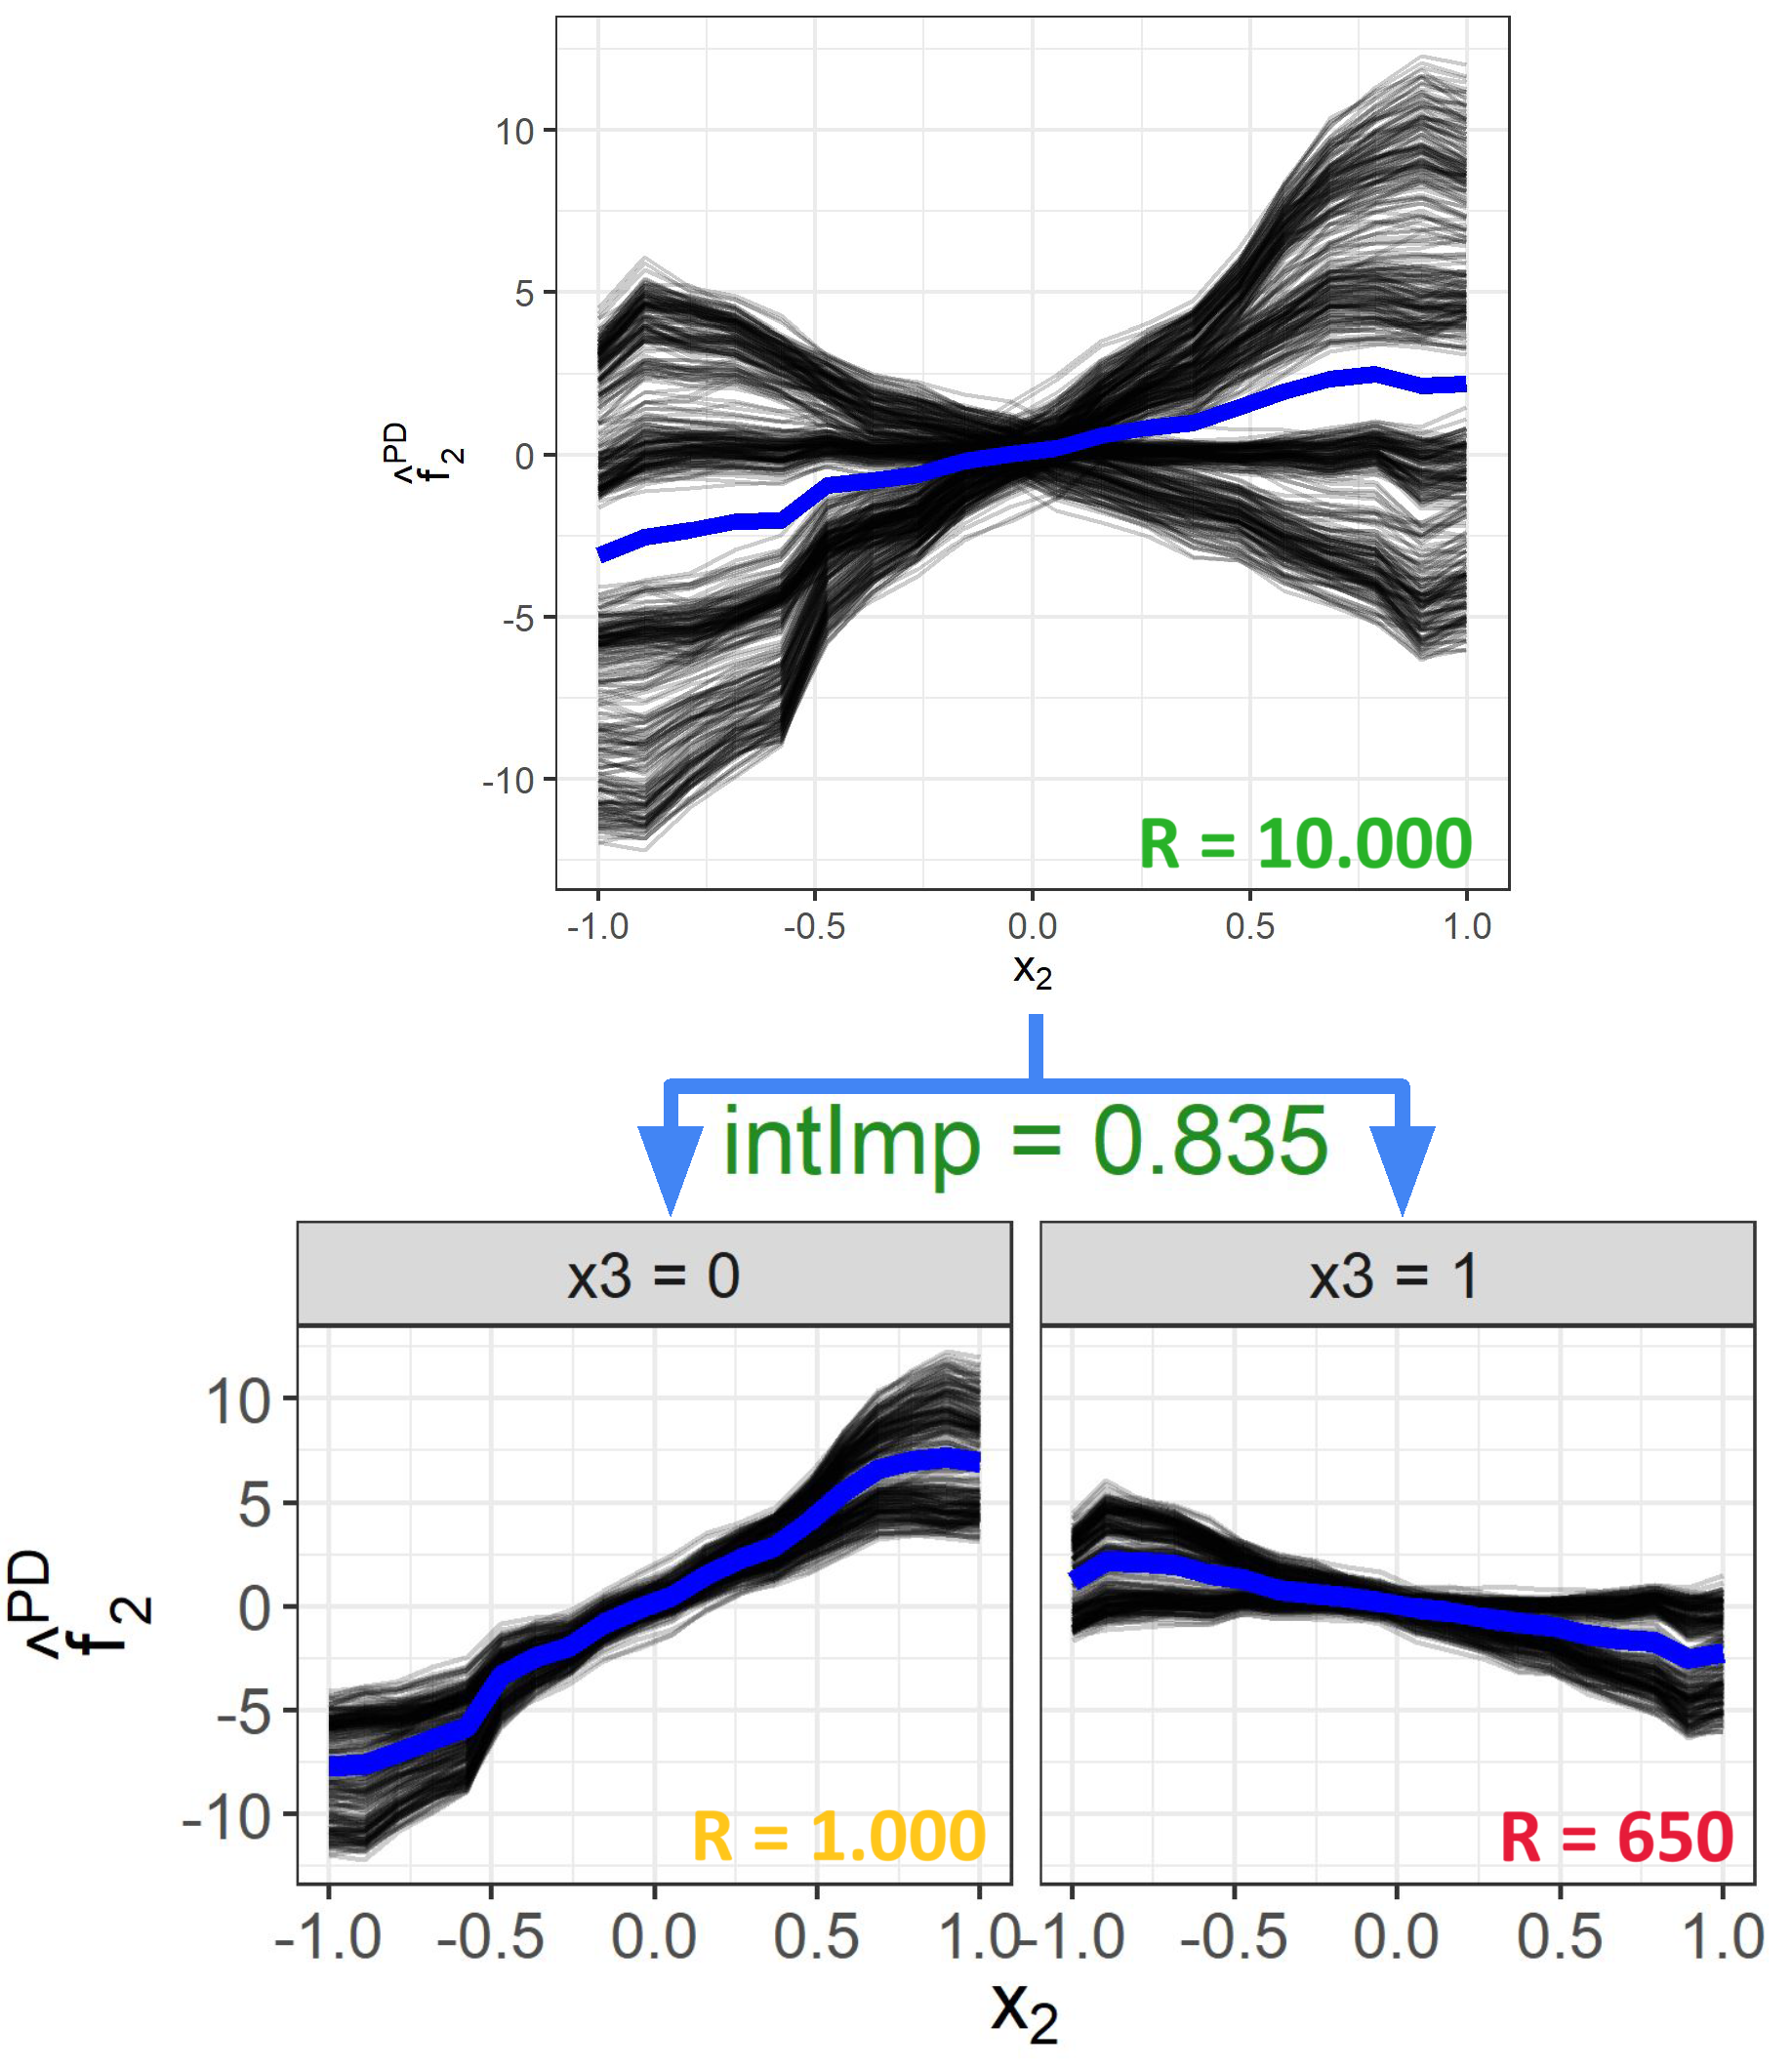
\includegraphics[width = 0.95\textwidth]{figure/sim1_fake.png}

Split reduces 83.5\% of variance.
    \end{column}
\end{columns}

\end{frame}


\begin{frame}{REPID Interaction Importance}
    
\begin{columns}[T, totalwidth=\textwidth]%, totalwidth=\textwidth]
    \begin{column}{0.53\textwidth}

\textbf{On feature level (for $x_j$):} 
%Relative interaction importance for feature $x_j$:
%We denote this subset by $\mathcal{B}_j \subset \mathcal{B}_P$ and the relative interaction importance by
\medskip

\centerline{$\textstyle
   intImp_j = \sum\nolimits_{i \in \mathcal{B}_j} intImp(\mathcal{N}_i)$}

\medskip

%\textbf{$\bm{intImp(\mathcal{N}_P)}$: risk reduction after one split relative to the root node risk}
%where $\mathcal{B}_j$ indexes parent nodes where splits are based on $x_j$.
where $\mathcal{B}_j$ indexes parent nodes split by $x_j$.

\medskip

\textbf{Interpretation:}
Overall reduction of ICE curve variance due to splits by $X_j$ (in \%).

\medskip

\textbf{Example:} For $X_1 \Rightarrow$  {\color{orange} $\mathcal{B}_1 = \{0, 2, 3\}$}
    \begin{center}
      \resizebox{1\textwidth}{!}{
\begin{tikzpicture}[scale=0.7, transform shape]
    \tikzset{treenode/.style={draw, rectangle, font=\LARGE}}
    \tikzset{line/.style={draw, thick}}

    % Root node
    \node [treenode, fill=orange] (a0) {$\mathcal{N}_0$};

    % Level 1 nodes
    \node [treenode, below=1cm of a0, xshift=-3cm] (a1) {$\mathcal{N}_1$};
    \node [treenode, fill=orange, below=1cm of a0, xshift=3cm] (a2) {$\mathcal{N}_2$};

    % Level 2 nodes
    \node [treenode, fill=orange, below=1cm of a1, xshift=-1.5cm] (a3) {$\mathcal{N}_3$};
    \node [treenode, below=1cm of a1, xshift=1.5cm] (a4) {$\mathcal{N}_4$};
    \node [treenode, below=1cm of a2, xshift=-1.5cm] (a5) {$\mathcal{N}_5$};
    \node [treenode, below=1cm of a2, xshift=1.5cm] (a6) {$\mathcal{N}_6$};

    % Level 3 nodes
    \node [treenode, below=1cm of a3, xshift=-0.75cm] (a7) {$\mathcal{N}_7$};
    \node [treenode, below=1cm of a3, xshift=0.75cm] (a8) {$\mathcal{N}_8$};
    \node [treenode, below=1cm of a4, xshift=-0.75cm] (a9) {$\mathcal{N}_9$};
    \node [treenode, below=1cm of a4, xshift=0.75cm] (a10) {$\mathcal{N}_{10}$};
    \node [treenode, below=1cm of a5, xshift=-0.75cm] (a11) {$\mathcal{N}_{11}$};
    \node [treenode, below=1cm of a5, xshift=0.75cm] (a12) {$\mathcal{N}_{12}$};
    \node [treenode, below=1cm of a6, xshift=-0.75cm] (a13) {$\mathcal{N}_{13}$};
    \node [treenode, below=1cm of a6, xshift=0.75cm] (a14) {$\mathcal{N}_{14}$};

    % Edges and labels
    \path [line] (a0.south) -- + (0,-0.5cm) -| (a1.north) node [pos=0.4, above, color=orange] {$X_1 < 5$};
    \path [line] (a0.south) -- + (0,-0.5cm) -| (a2.north) node [pos=0.4, above, color=orange] {$X_1 \geq 5$};

    \path [line] (a1.south) -- + (0,-0.5cm) -| (a3.north) node [pos=0.3, above, yshift = -0.05cm] {$X_2 < 3$};
    \path [line] (a1.south) -- + (0,-0.5cm) -| (a4.north) node [pos=0.3, above, yshift = -0.05cm] {$X_2 \geq 3$};

    \path [line] (a2.south) -- + (0,-0.5cm) -| (a5.north) node [pos=0.3, above, color=orange, yshift = -0.05cm] {$X_1 < 7$};
    \path [line] (a2.south) -- + (0,-0.5cm) -| (a6.north) node [pos=0.3, above, color=orange, yshift = -0.05cm] {$X_1 \geq 7$};

    \path [line] (a3.south) -- + (0,-0.5cm) -| (a7.north) node [pos=0.5, above, color=orange, yshift = -0.05cm] {\small $X_1 < 2$};
    \path [line] (a3.south) -- + (0,-0.5cm) -| (a8.north) node [pos=0.5, above, color=orange, yshift = -0.05cm] {\small $X_1 \geq 2$};

    \path [line] (a4.south) -- + (0,-0.5cm) -| (a9.north) node [pos=0.5, above, yshift = -0.05cm] {\small $X_3 < 4$};
    \path [line] (a4.south) -- + (0,-0.5cm) -| (a10.north) node [pos=0.5, above, yshift = -0.05cm] {\small $X_3 \geq 4$};

    \path [line] (a5.south) -- + (0,-0.5cm) -| (a11.north) node [pos=0.5, above, yshift = -0.05cm] {\small $X_2 < 5$};
    \path [line] (a5.south) -- + (0,-0.5cm) -| (a12.north) node [pos=0.5, above, yshift = -0.05cm] {\small $X_2 \geq 5$};

    \path [line] (a6.south) -- + (0,-0.5cm) -| (a13.north) node [pos=0.5, above, yshift = -0.05cm] {\small $X_4 < 7$};
    \path [line] (a6.south) -- + (0,-0.5cm) -| (a14.north) node [pos=0.5, above, yshift = -0.05cm] {\small $X_4 \geq 7$};

\end{tikzpicture}}
    \end{center}
    \end{column}
\pause
    \begin{column}{0.54\textwidth}


    \centering
    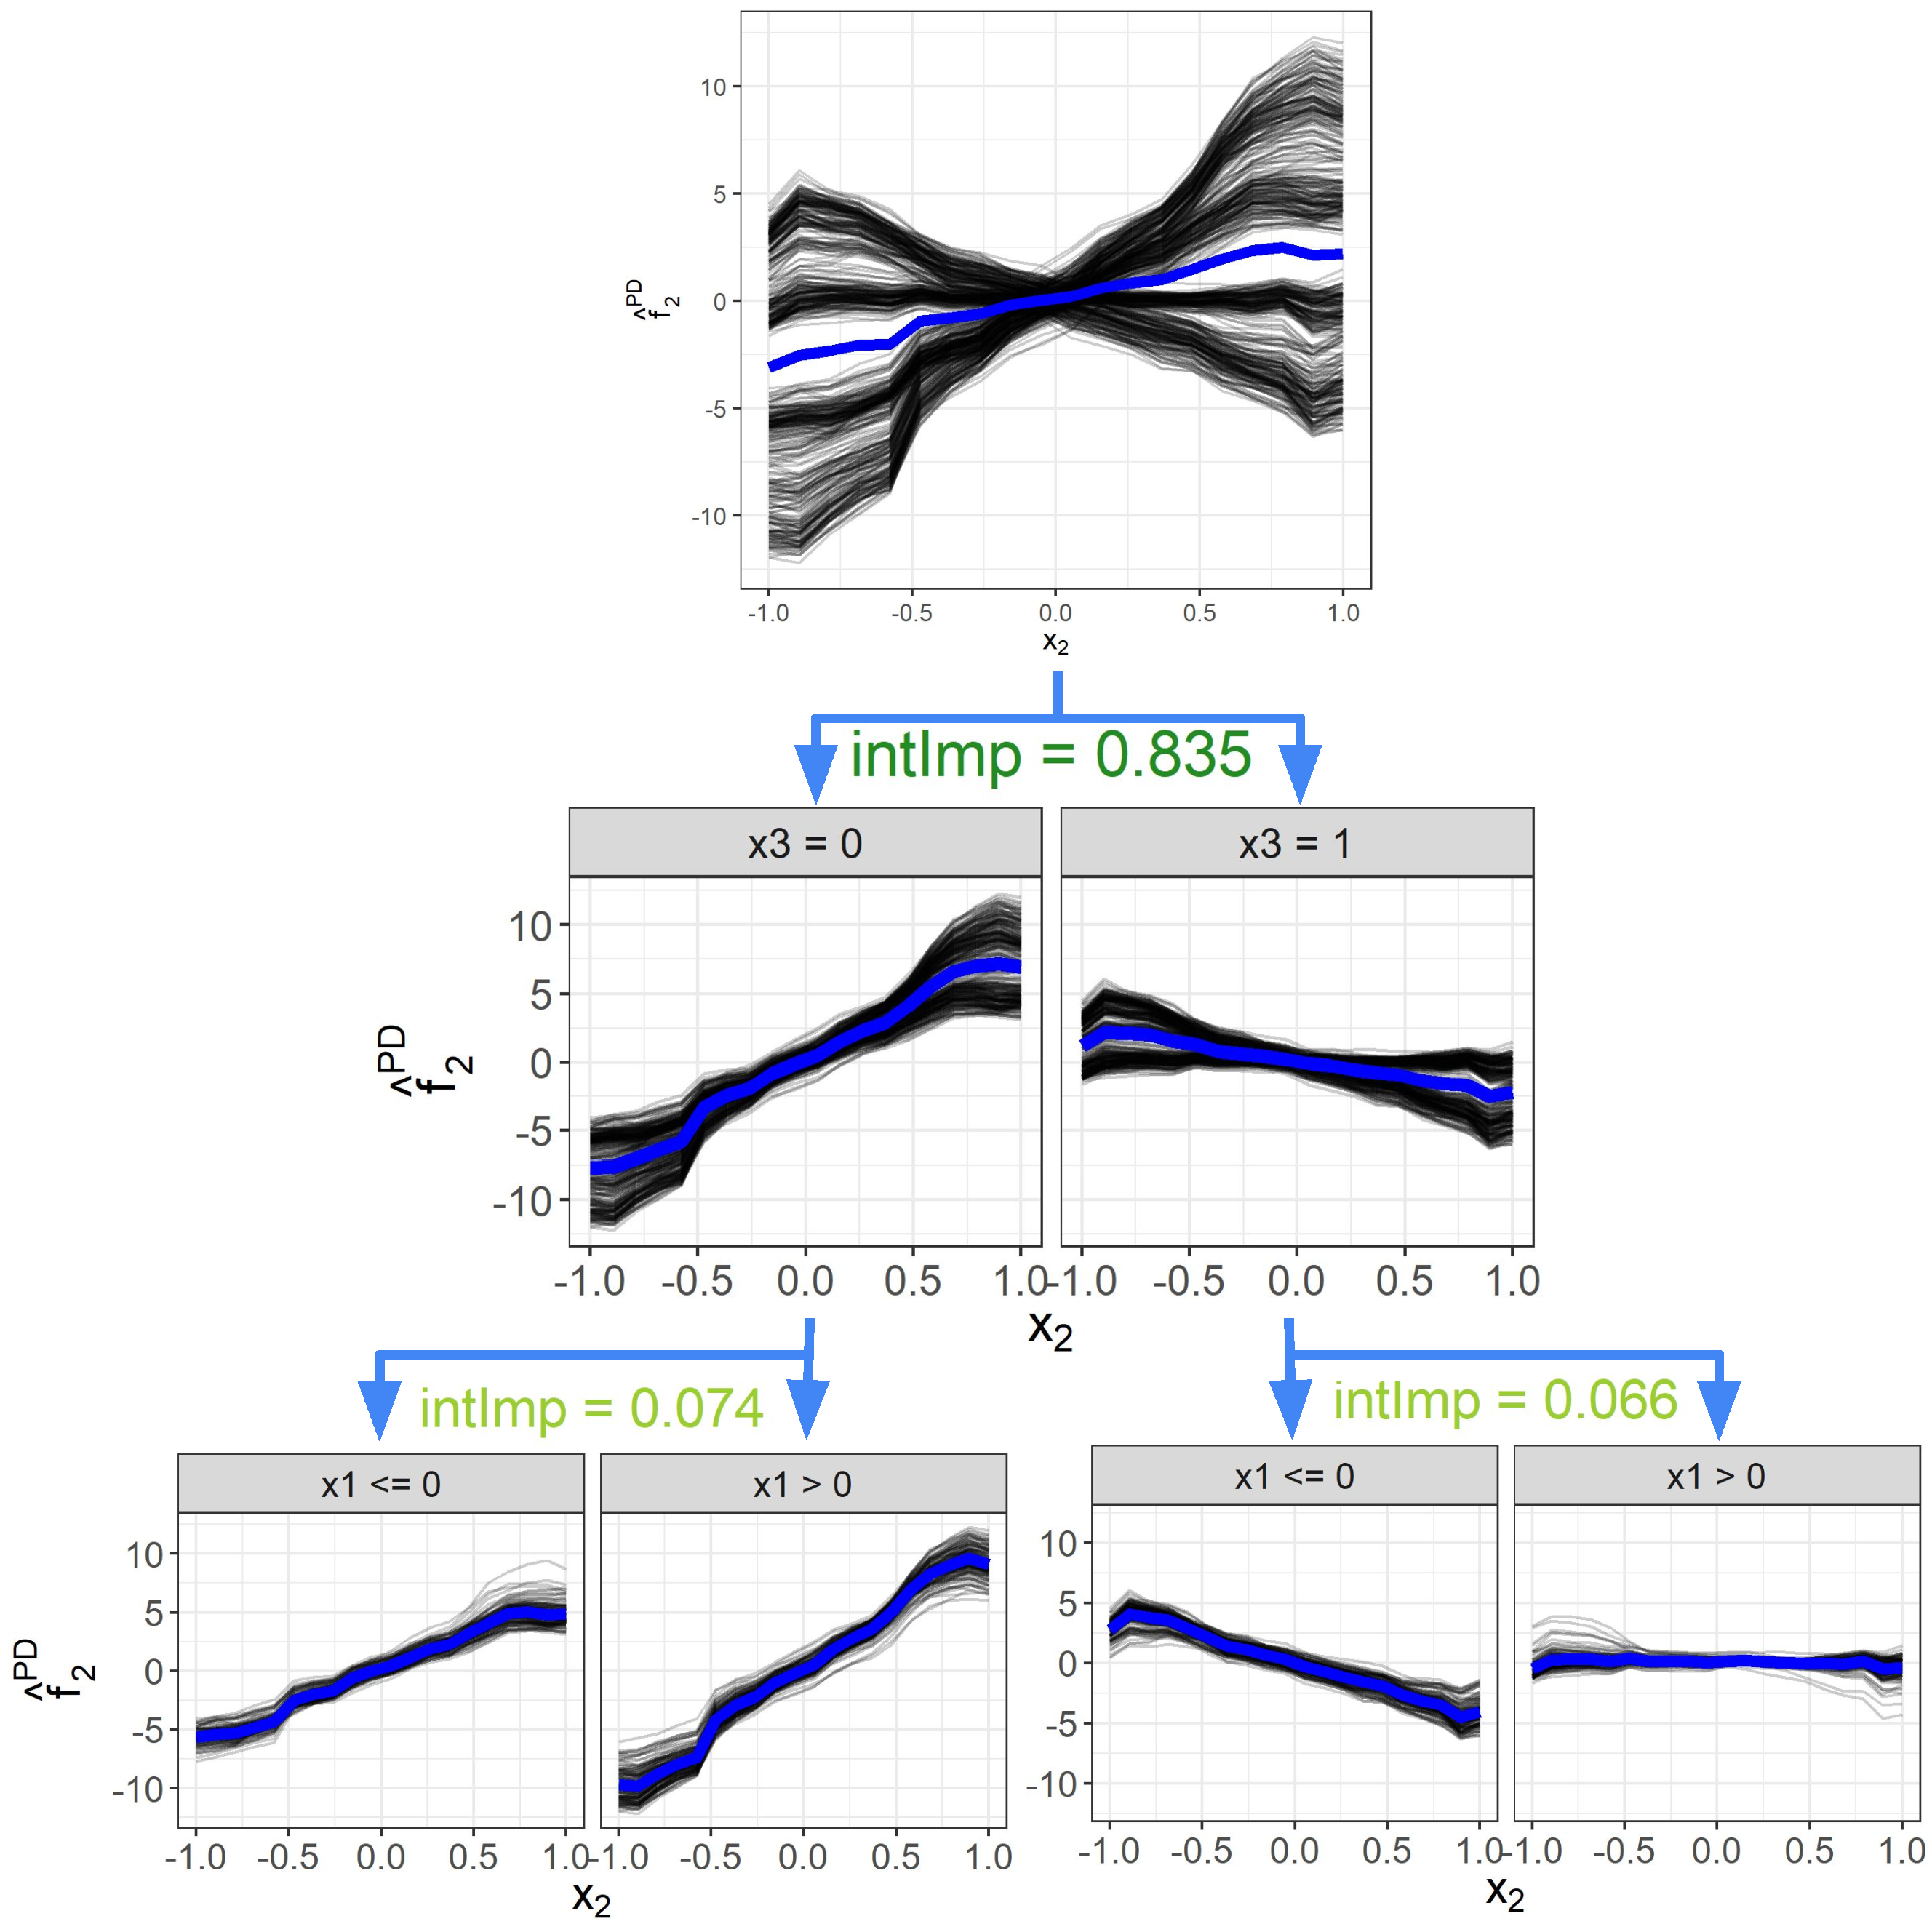
\includegraphics[width=\textwidth]{figure/sim1}
    
    \textbf{Note:} \textit{intImp} can also be used as a stopping criterion.
     %\begin{minipage}[t]{.5\textwidth}
    %   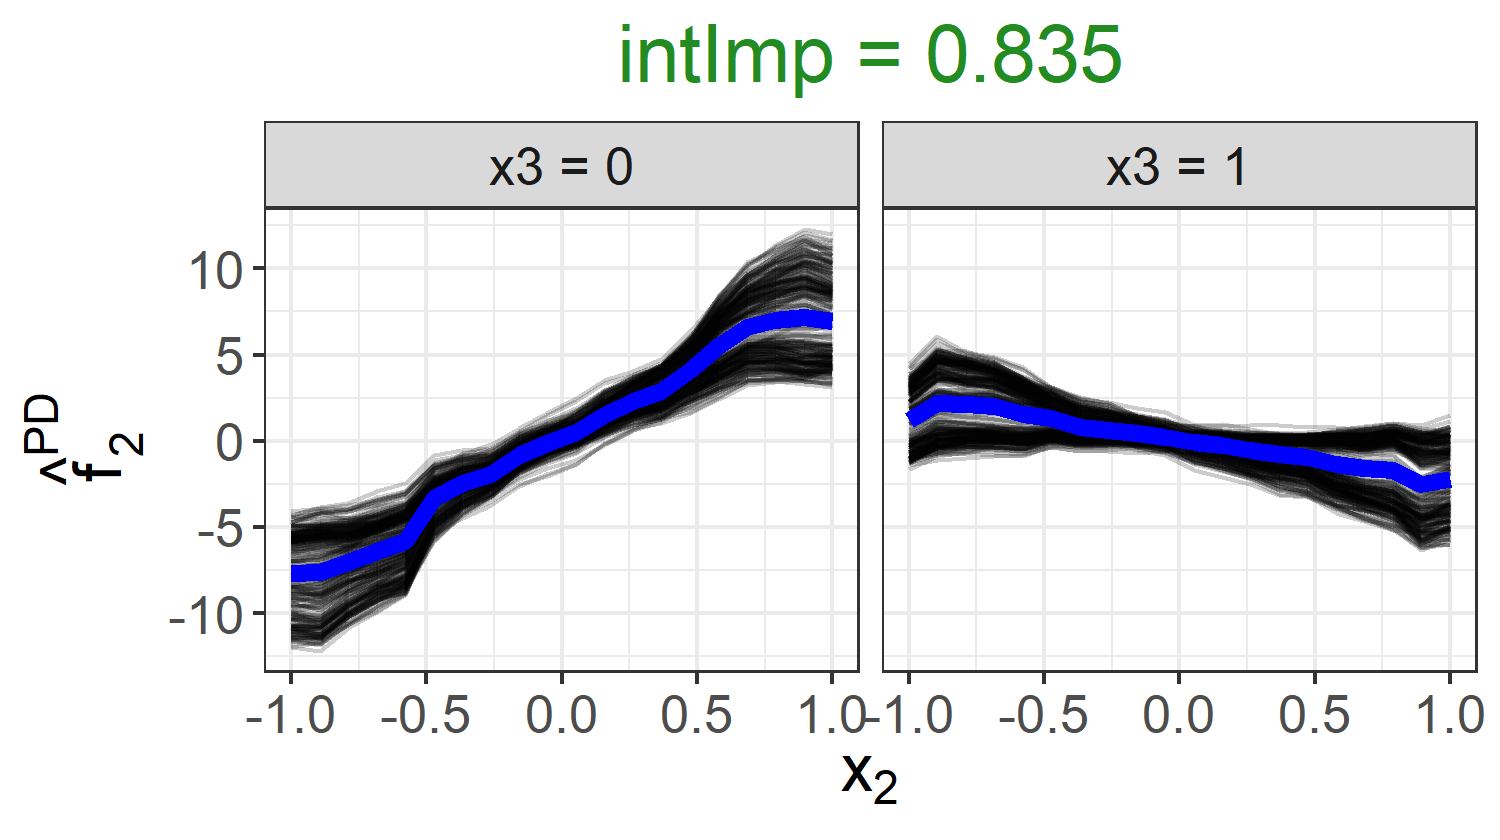
\includegraphics[width=0.37\textwidth]{figure/sim1_dt_split1.png}
    %   \scalebox{1}{
    %   \hspace{15pt} 
    %   \begin{tikzpicture}
    %   \usetikzlibrary{arrows}
    %     \usetikzlibrary{shapes}
    %      \tikzset{treenode/.style={draw}}
    %      \tikzset{line/.style={draw, thick}}
    %     \node [treenode](a0) {} ; [below=1pt,at=(4,0)]  {};
    %      \node [treenode, below=0.3cm, at=(a0.south), xshift=-1.3cm]  (a1) {};
    %      \node [treenode, below=0.3cm, at=(a0.south), xshift=-0.2cm]  (a2) {};
    %      \path [line] (a0.south) -- + (0,-0.2cm) -| (a1.north) node [midway, above] {};
    %      \path [line] (a0.south) -- +(0,-0.2cm) -|  (a2.north) node [midway, above] {};
    %   \end{tikzpicture}
    %   \hspace{25pt}
    %   \begin{tikzpicture}
    %   \usetikzlibrary{arrows}
    %     \usetikzlibrary{shapes}
    %      \tikzset{treenode/.style={draw}}
    %      \tikzset{line/.style={draw, thick}}
    %     \node [treenode] (a01) {};[below=5pt,at=(node1.south) , xshift=0cm]
    %      \node [treenode, below=0.3cm, at=(a01.south), xshift=0.1cm]  (a1) {};
    %      \node [treenode, below=0.3cm, at=(a01.south), xshift=1.1cm]  (a2) {};
    %      \path [line] (a01.south) -- + (0,-0.2cm) -| (a1.north) node [midway, above] {};
    %      \path [line] (a01.south) -- +(0,-0.2cm) -|  (a2.north) node [midway, above] {};
    %   \end{tikzpicture}
    %   }
    % 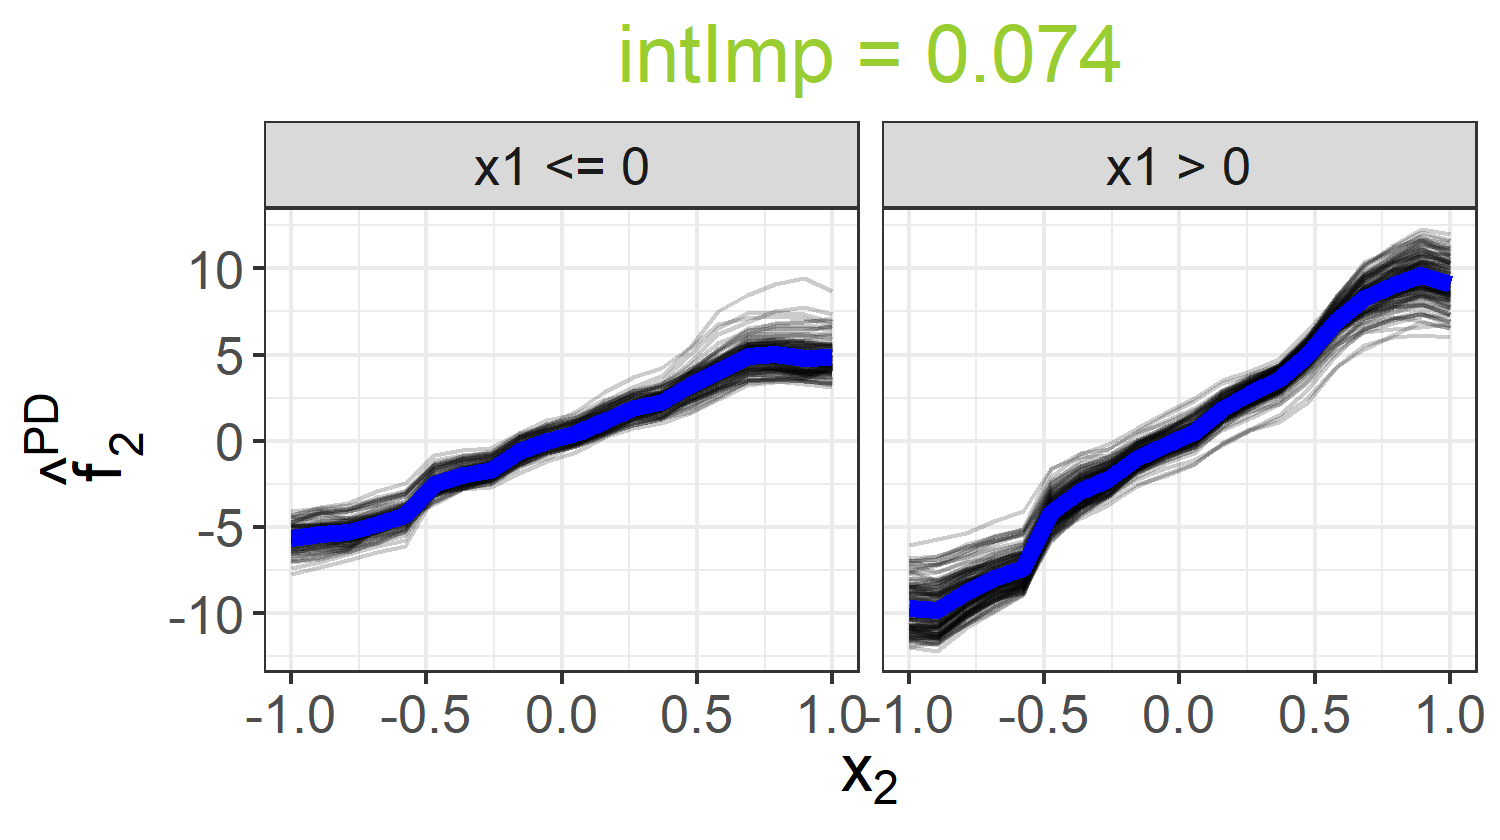
\includegraphics[width=0.37\textwidth]{figure/sim1_dt_split2_1.png}
    % 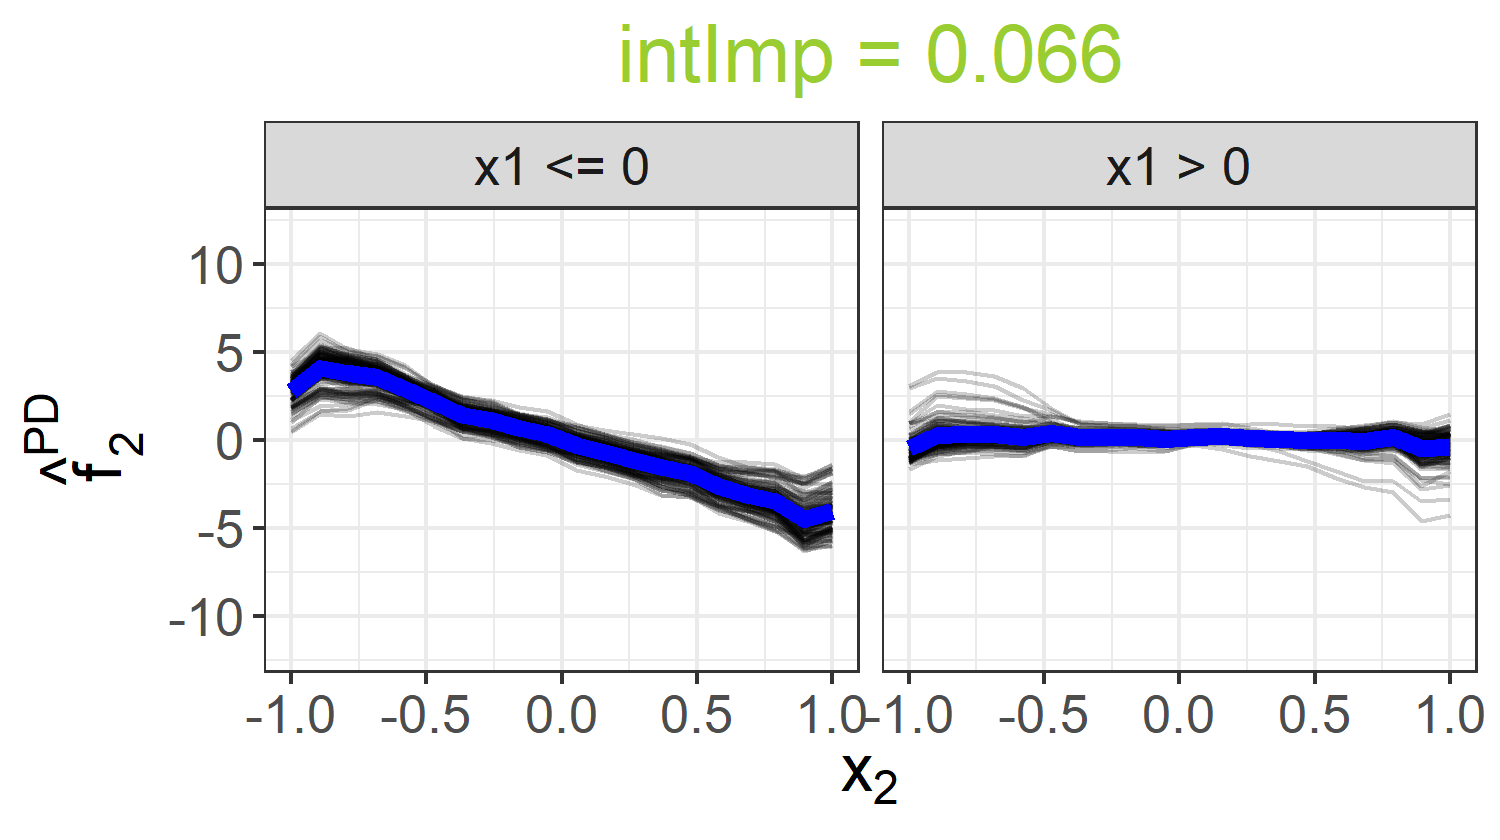
\includegraphics[width=0.37\textwidth]{figure/sim1_dt_split2_2.png}
    
 \vspace{-200px}
    \scriptsize
 \hspace{130px}
 \setlength{\tabcolsep}{1pt}
 \begin{tabular}{|c|c|}
    \hline
       $x_j$ & $intImp_j$  \\\hline
       \rowcolor{ForestGreen!70}
        $\xv_3$     & 0.835 \\
        \rowcolor{YellowGreen!50}
        $\xv_1$     &  0.14\\\hline
    \end{tabular}\\
 \hspace{138px}= 0.975
      %\footnotesize\\
    %\vspace{150px}

    \end{column}

\end{columns}

\end{frame}





\begin{frame}{Outperforming SOTA}

\textbf{Simulation setting}
\begin{itemize}
    \item Draw 1000 i.i.d. samples from $X_1, \ldots , X_4 \sim \mathcal{U}(-1,1)$
    \item True underlying function: $f(\xv) = \sum\nolimits_{j=1}^4 \xv_j + \xv_1 \xv_2 + \xv_2 \xv_3 + \xv_1 \xv_3 + \xv_1 \xv_2 \xv_3 + \epsilon$ % , \epsilon \sim \mathbbm{N}(0, 0.01 \sigma(\mu(\xv))^2)
    \item Fit a correctly specified linear model (interactions with $\xv_4$ are excluded)
    \item 30 reps, measure interaction strength between $\xv_2$ and all other 3 features
\end{itemize}

\textbf{Which methods are sensitive to changes in main effect sizes or feature correlations?}


    \begin{table}[thb]
\vspace{.1in}
    \label{tab:simSummary}
    \begin{center}
    \begin{tabular}{|p{5.4cm}|p{1.6cm}|p{1.8cm}|p{1.6cm}|p{1.6cm}|}
    \hline
       Pitfall & REPID & H-Statistic & Greenwell & SHAP  \\\hline
       sensitive to changes of main effect & No & Yes & Yes & No\\\hline
       sensitive to changes of correlation between $\xv_j$ and other features & No & Yes & No & Yes\\
  \hline
    \end{tabular}
    \end{center}
\end{table}
\vspace*{0.2cm}




\end{frame}

\begin{frame}{Outperforming SOTA}
\centerline{
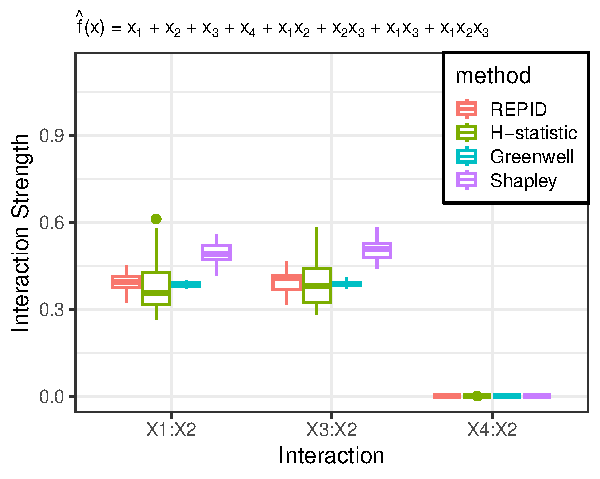
\includegraphics[width=0.4\textwidth, page = 1]{figure/sim_sensi_linear.pdf}
\includegraphics[width=0.4\textwidth, page = 2]{figure/sim_sensi_linear.pdf}
}

   \begin{itemize}
       \item \textbf{Left (initial setting)}: Interaction strength of $\xv_1$:$\xv_2$ and $\xv_3$:$\xv_2$ similar; $\xv_4$:$\xv_2$ no interaction
       \item \textbf{Right}: Set main effect $\beta_1$ = 0.1
       
   \begin{itemize}
       \item \textbf{Expectation}: Interaction strengths should not change
       \item \textbf{Fail}: H-statistic ($\xv_1$:$\xv_2$ > $\xv_3$:$\xv_2$) and Greenwell ($\xv_1$:$\xv_2$ < $\xv_3$:$\xv_2$) 
   \end{itemize}
   \end{itemize}
\end{frame}

\begin{frame}{Outperforming SOTA}
\centerline{
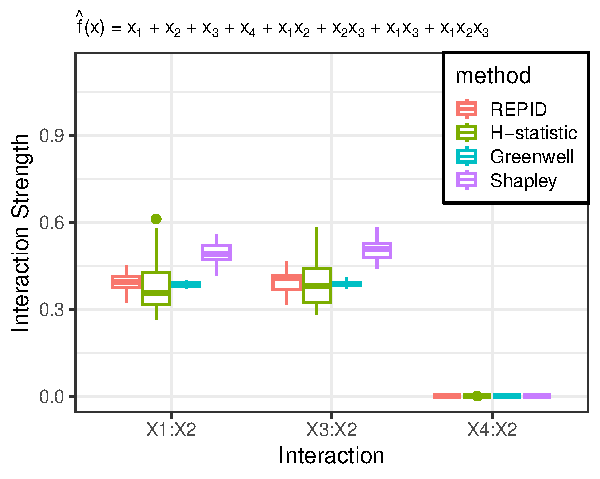
\includegraphics[width=0.4\textwidth, page = 1]{figure/sim_sensi_linear.pdf}
\includegraphics[width=0.4\textwidth, page = 3]{figure/sim_sensi_linear.pdf}
}
  \begin{itemize}
        \item \textbf{Left (initial setting)}: Interaction strength of $\xv_1$:$\xv_2$ and $\xv_3$:$\xv_2$ similar; $\xv_4$:$\xv_2$ no interaction
       \item \textbf{Right}: Increase correlation $\rho(\xv_1, \xv_2) = 0.9$
          \begin{itemize}
       \item \textbf{Expectation}: Interaction strengths should not change
       \item \textbf{Fail}: H-statistic ($\xv_1$:$\xv_2$ < $\xv_3$:$\xv_2$) and Shapley ($\xv_1$:$\xv_2$ > $\xv_3$:$\xv_2$)
   \end{itemize}
       \item[$\rightarrow$] \textbf{REPID is the only method which always leads to correct rankings for these settings}  
   \end{itemize}
   
\end{frame}



\begin{frame}{Limitations of REPID}

\begin{columns}[T, totalwidth = \textwidth]
    \begin{column}{0.6\textwidth}

%\pause
% \textbf{Limitations}:
      \begin{itemize}
  \item[1)] Restricted to one feature of interest \\
  $\Rightarrow$ Different regions for different features \\
  %$\Rightarrow$ No unique decomposition of $\hat{f}(x)$\\%iction function possible\\
  %\item Restricted to ICE curves and PDs $\rightarrow$ not flexible w.r.t. feature effect method
  %\pause
  \item<2->[2)] Restricted to PD (global) and ICE (local) as feature effect methods\\
  $\Rightarrow$ Inherits extrapolation problem\\
  %\phantom{$\Rightarrow$} 
  (unlikely combinations of feature values)
      %\item Feature effect methods based on integrating over marginal distributions such as ICE and PD might extrapolate in unseen or sparse regions (e.g., small $\xv_1$ and high $\xv_3$ values)
      %\item Global/regional effects are not representative w.r.t. the data distribution  
   \item<2->[$\leadsto$] Follow-up GADGET %``Generalized Additive Decomposition of Global feature EffecTs based on interactions'' 
[under review]
  \end{itemize}


        % \begin{itemize}
        %     \item $f(X) = 3X_1\mathbbm{1}_{X_3>0} - 3X_1\mathbbm{1}_{X_3\leq 0} + X_3 + \epsilon$
        %     \item Features uniformly distributed
        %     \item Left: features independent
        %     \item Right: $X_1$ and $X_3$ highly correlated
        %     \item First split: $\xv_3 \leq 0$ (blue) and $\xv_3 > 0$ (orange)
        % \end{itemize}
    \end{column}

    \only<1>{   \begin{column}{0.52\textwidth}
    \centering
    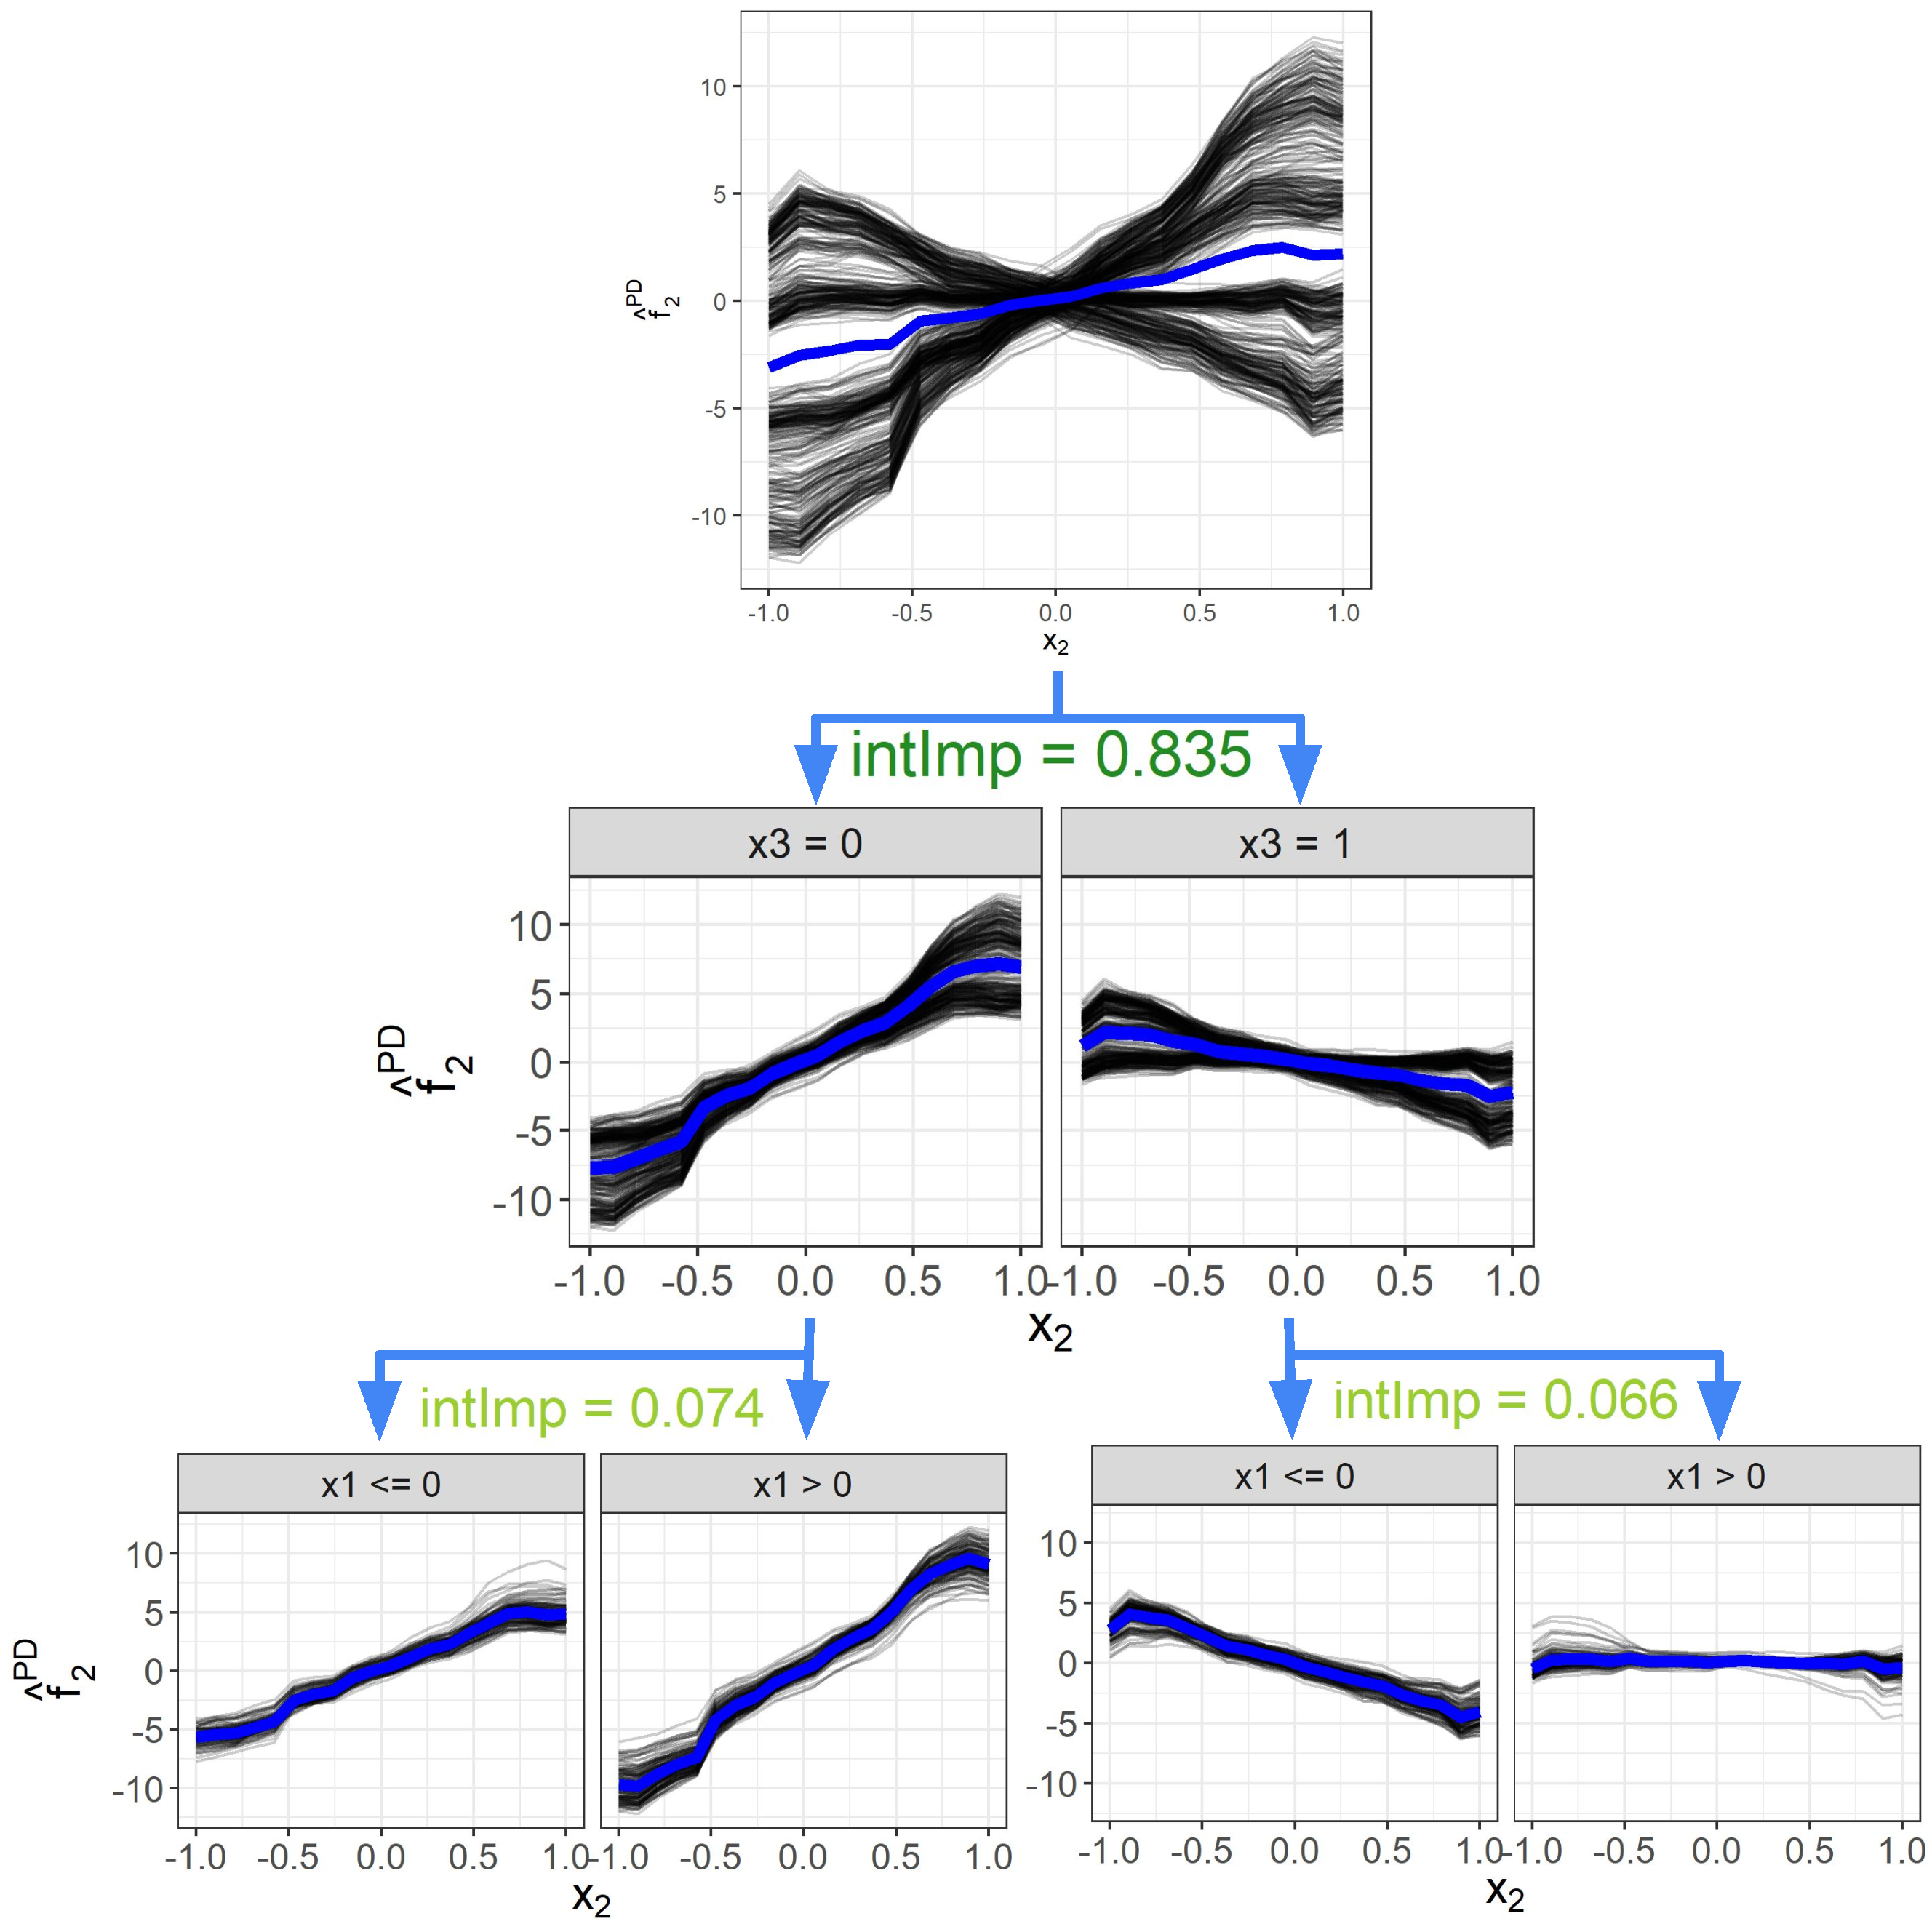
\includegraphics[width=0.95\textwidth]{figure/sim1}
    \vspace{-8pt}
        \begin{columns}[T, totalwidth = \linewidth]
     \footnotesize
            \begin{column}{0.125\linewidth}
            \centering
             $\hat{f}_2^{PD}(X_2)$ %, X_1 > 0 \land X_3 = 0\)\\
         \end{column}
         \begin{column}{0.175\linewidth}
         \centering
             $\approx 8X_2$ %, X_1 > 0 \land X_3 = 0\)\\
         \end{column}
        \begin{column}{0.225\linewidth}
\centering
            $\approx 16X_2$ %, X_1 \leq 0 \land X_3 = 0\)
         \end{column}
        \begin{column}{0.225\linewidth}
        \centering
            $ \approx -8X_2$ %, X_1 \leq 0 \land X_3 \neq 0\)
         \end{column}        
         \begin{column}{0.225\linewidth}
         \centering
             $\approx 0$%, X_1 > 0 \land X_3 \neq 0\)\\
         \end{column}
        \begin{column}{0.025\linewidth}

         \end{column}
     \end{columns}
    \end{column}
}
    \only<2->{\begin{column}{0.52\textwidth}
        %\begin{figure}
      %   \hspace{0.025\linewidth} uncorrelated \hspace{0.225\linewidth} correlated \hspace{0.2\linewidth}
      % \includegraphics[width = \textwidth]{figure/example_repid_extrapol.pdf}
      %      $f(X) = \highlight{3X_1\mathbbm{1}_{X_3>0}} \highlightICE{- 3X_1\mathbbm{1}_{X_3\leq 0}} + X_3 + \epsilon$
      %      \begin{itemize}
      %          \item Left: $X_1, X_2, X_3 \sim \mathbbm{U}(-1,1)$ iid
      %          \item Right: $X_1 = X_3 + \epsilon_1, \epsilon_1 \sim \mathbbm{N}(0, 0.0625)$
      %          \item Model: Tuned feedforward NN
      %          \item Split: $X_3 \leq 0$ (blue), $X_3 > 0$ (orange)
      %      \end{itemize}
      \centering
 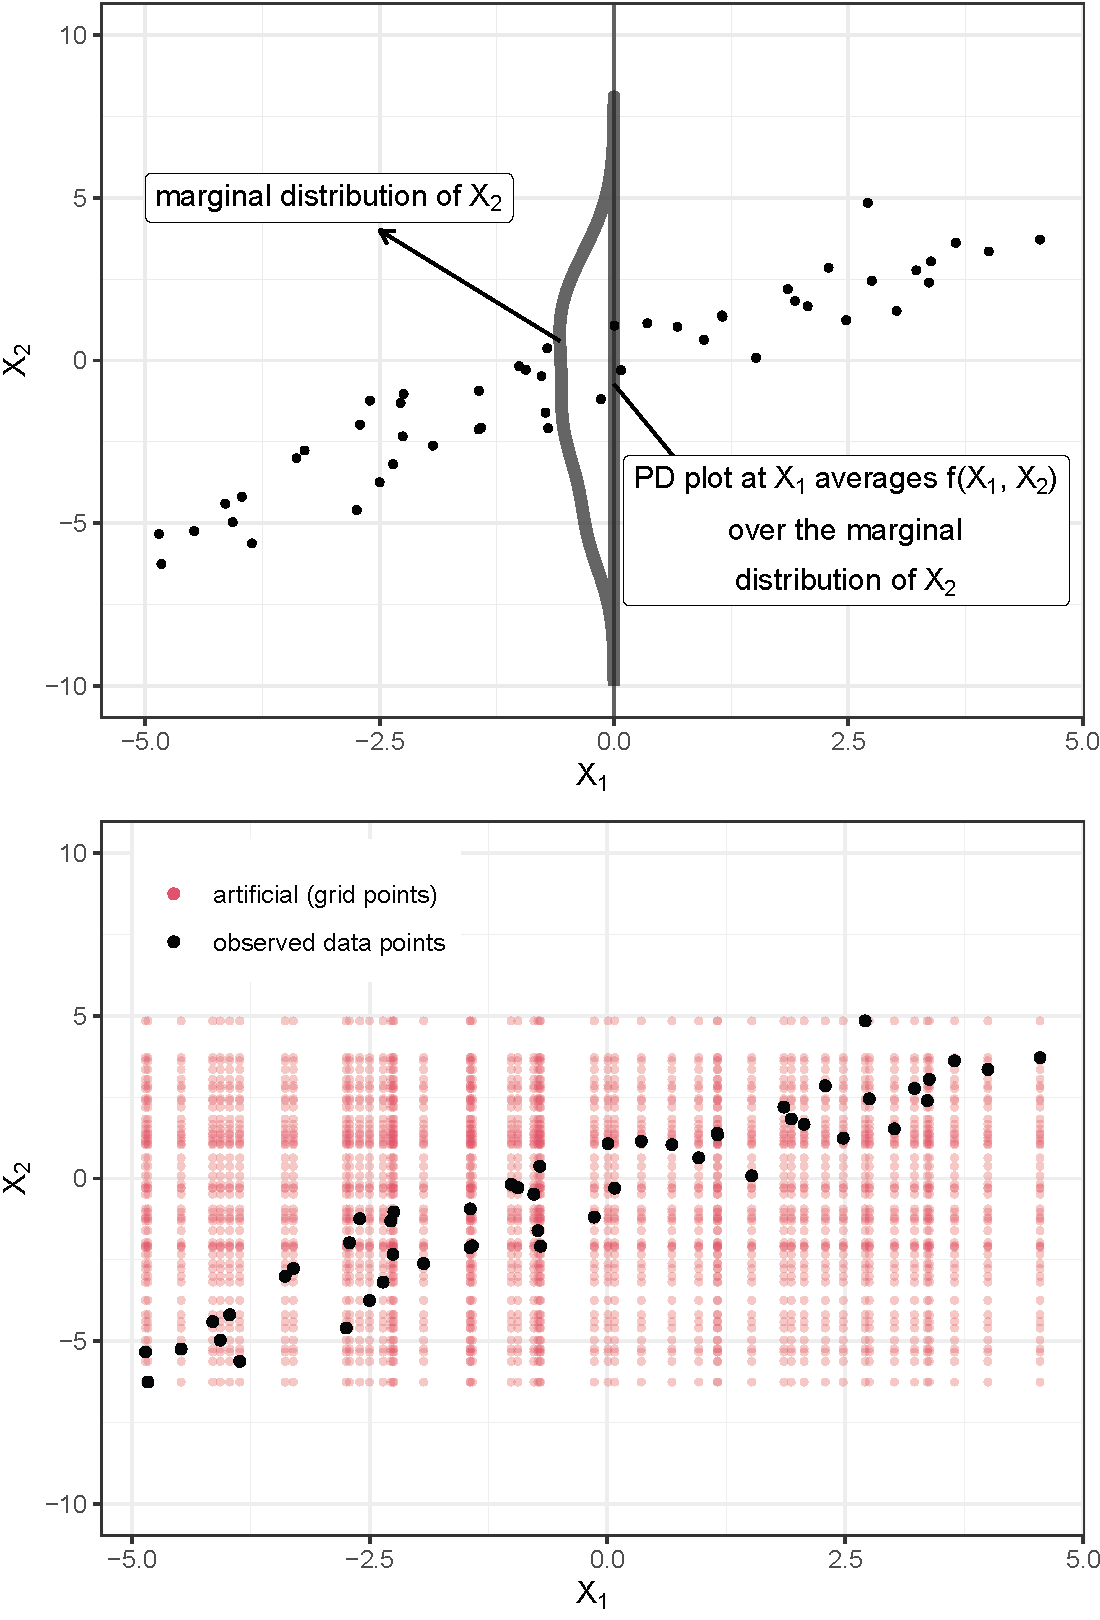
\includegraphics[width = 0.675
 \textwidth]{figure/ale_pdplot.png}
     % \caption{
      %$X_1, X_2, X_3 \sim \mathbbm{U}(-1,1)$ and 
      %$Y = 3X_1\mathbbm{1}_{X_3>0} - 3X_1\mathbbm{1}_{X_3\leq 0} + X_3 + \epsilon$% with $\epsilon \sim \mathbb{N}(0,0.09)$. 
      %left: features independent, right: $X_1$ and $X_3$ highly correlated.
      %$X_1 = X_3 + \delta$ and $\delta \sim \mathbb{N}(0, 0.0625)$. 
      %First split: $\xv_3 \leq 0$ (blue) and $\xv_3 > 0$ (orange).}
  %\end{figure}
    \end{column}}

\end{columns}
\bigskip
\end{frame}


\begin{frame}{Conclusion}

\begin{columns}[T, totalwidth = \textwidth]
    \begin{column}{0.58\textwidth}

 \textbf{Summary of Contributions (REPID)}:
 \begin{itemize}
    \item Regional effects in interpretable regions
    \item Additive decomp. of feature effect 
    %\item Prove meaningfulness of objective - only feature interactions between $\xv_j$ and $\xv_{-j}$ minimized %(measures only feature interactions)
    \item Quantify feature interactions 
    \item Outperforms SOTA interaction indices
    %H-Statistics, Greenwell's and Shapley
\end{itemize}

 \textbf{Summary of Contributions (GADGET)}:
 \begin{itemize}
 \item Unique regions for multiple features
 \item Additive decomp. of prediction function%\\
 \item Extension to ALE and Shapley Dependence
% $\Rightarrow$ TODO: Investigate usefulness as ``approximation'' when terminal regions contain interactions
 \item Test to identify significant interactions
\end{itemize}

        % \begin{itemize}
        %     \item $f(X) = 3X_1\mathbbm{1}_{X_3>0} - 3X_1\mathbbm{1}_{X_3\leq 0} + X_3 + \epsilon$
        %     \item Features uniformly distributed
        %     \item Left: features independent
        %     \item Right: $X_1$ and $X_3$ highly correlated
        %     \item First split: $\xv_3 \leq 0$ (blue) and $\xv_3 > 0$ (orange)
        % \end{itemize}
    \end{column}
    \begin{column}{0.45\textwidth}
    \centering
    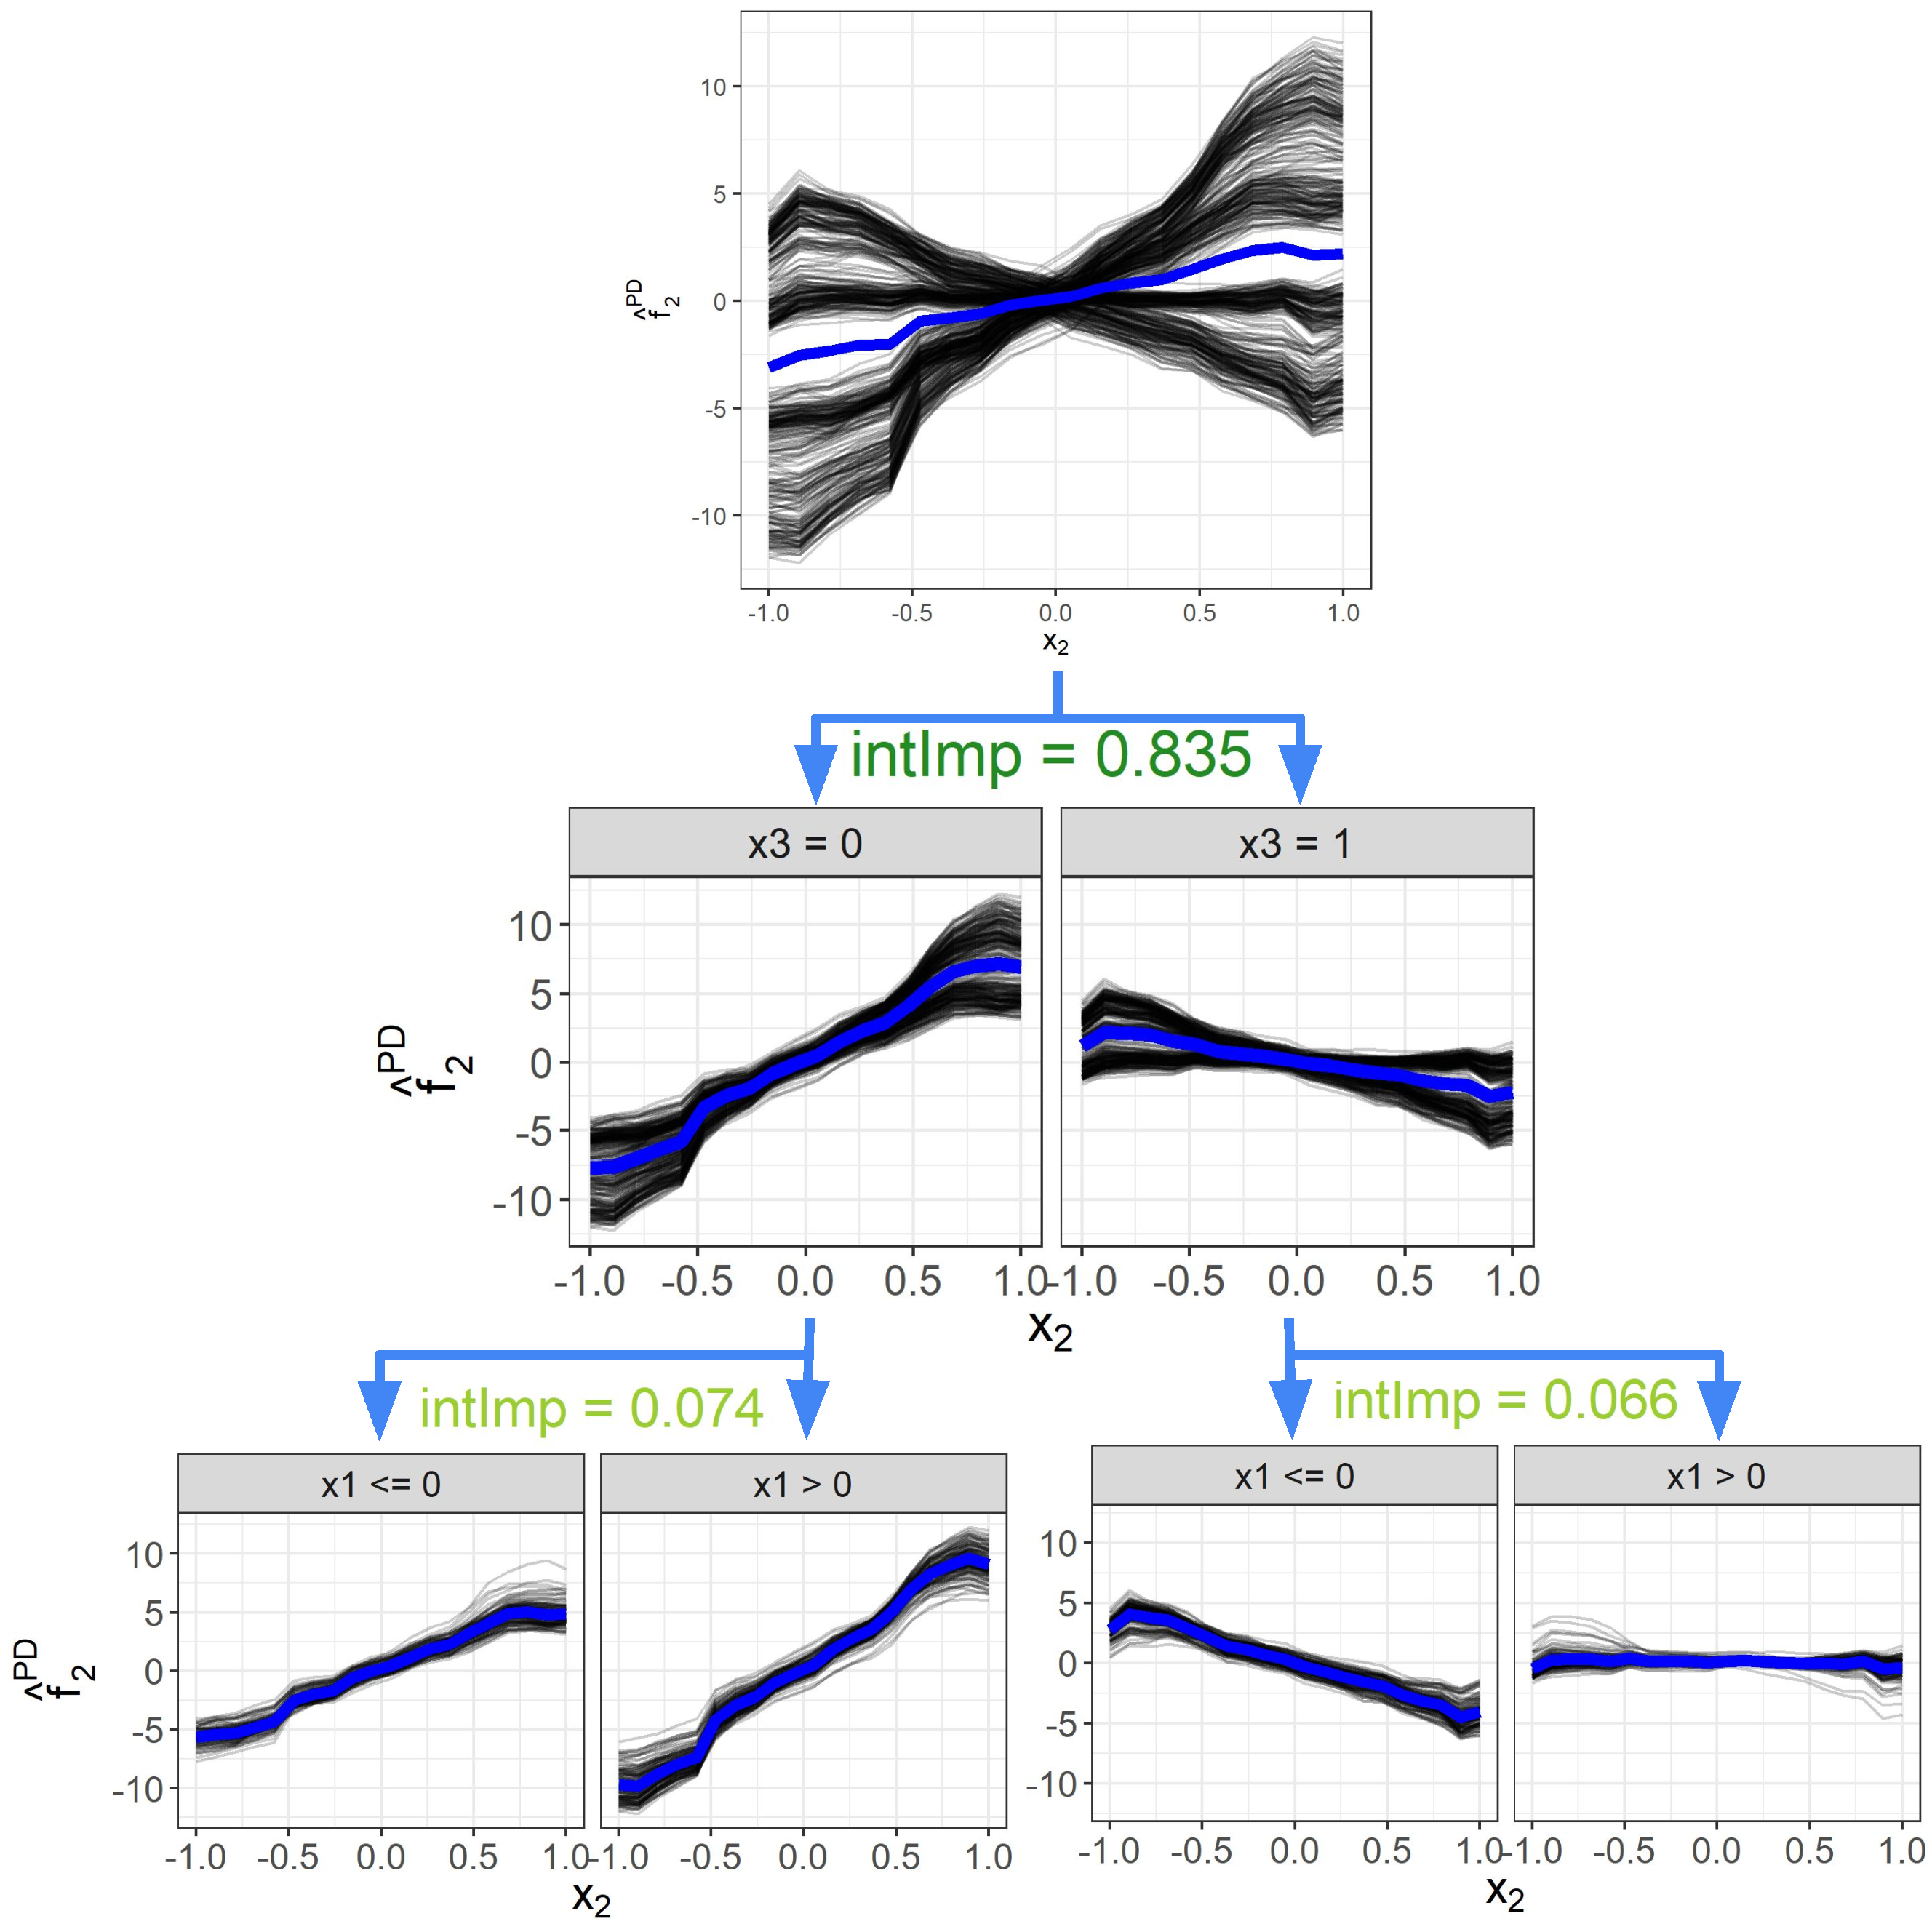
\includegraphics[width=0.95\textwidth]{figure/sim1}
    \vspace{-8pt}
        \begin{columns}[T, totalwidth = \linewidth]
     \footnotesize
            \begin{column}{0.125\linewidth}
            \centering
             $\hat{f}_2^{PD}(X_2)$ %, X_1 > 0 \land X_3 = 0\)\\
         \end{column}
         \begin{column}{0.175\linewidth}
         \centering
             $\approx 8X_2$ %, X_1 > 0 \land X_3 = 0\)\\
         \end{column}
        \begin{column}{0.225\linewidth}
\centering
            $\approx 16X_2$ %, X_1 \leq 0 \land X_3 = 0\)
         \end{column}
        \begin{column}{0.225\linewidth}
        \centering
            $ \approx -8X_2$ %, X_1 \leq 0 \land X_3 \neq 0\)
         \end{column}        
         \begin{column}{0.225\linewidth}
         \centering
             $\approx 0$%, X_1 > 0 \land X_3 \neq 0\)\\
         \end{column}
        \begin{column}{0.025\linewidth}

         \end{column}
     \end{columns}
    \end{column}

\end{columns}

\medskip
\textbf{Further Directions}: 

Pruning, GADGET as a predictor, comparing regions across models, efficient implementation, more efficient testing and splitting approach, $\dots$
\bigskip
\end{frame}




\endlecture
\end{document}

